%! TeX program = lualatex
%---------------------------ALLGEMEINE IMPORTS-------------------------------------
\documentclass[12pt,english,ngerman]{scrartcl}

\usepackage{iftex}

% text input and font
\ifluatex  % LuaLaTeX
    \usepackage{fontspec}
    % main font automatically: Latin Modern
    %\setmonofont{Consolas}
    % \newfontfamily{\Consolas}{Consolas}
\else  % pdfLaTeX
    \usepackage[utf8]{inputenc}  % input in UTF-8
    \usepackage[T1]{fontenc}  % output in T1 fonts (west European encoding)
    \usepackage{lmodern}  % Latin modern font for main text
    \usepackage[mono]{zi4}  % Consolas font for monospaced text
    % \newfontfamily{\Consolas}{\fontfamily{zi4}}
\fi

% text processing
\usepackage{babel}  % language package
\usepackage[intlimits]{mathtools}  % upgrade of amsmath (automatically loaded) - \int^_ like \limits^_
\usepackage{amssymb}  % upgrade of amsfonts (American Math Society)
\usepackage{amstext}  % \text command in math environments
%\usepackage{bm}  % bold math fonts
% \LetLtxMacro{\svqty}{\qty}
% \usepackage{physics}  % macros for easier typesetting of physical formulas
% \LetLtxMacro{\qty}{\svqty}
\usepackage{letltxmacro}  % \let command for robust macros (new sqrt)
\usepackage{chemformula}  % typeset chemical formulas
\usepackage{microtype}


% page geometry
\usepackage{scrlayer-scrpage}  % page formatting with KOMA options
\usepackage[paper=a4paper, hmargin=3cm, vmargin=2.5cm, includehead, includefoot, head=29pt]{geometry}  % horizontal: 3cm, vertical: 2.5cm strict with or without headers and footers
\usepackage{tabto}  % tab stops
\NumTabs{8}  % 8 equally spaced of \textwidth tab stops



% floats
\usepackage[hypcap=false, labelfont=bf]{caption, subcaption}  % caption editing - hypcap warning with hyperref
\usepackage{float}  % for [H] (forced here) specifier
\usepackage{tabularray}
\usepackage{diagbox}  % table cells with diagonal lines


% graphical input
\usepackage{graphicx}  % input JPEG, PNG, PDF, etc.
\usepackage{pdfpages}  % input PDF as whole pages
\usepackage{lastpage}  % reference to last page
\usepackage{pgfplots}  % for tikzplotlib
\usepgfplotslibrary{groupplots,dateplot}
\usetikzlibrary{patterns,shapes.arrows}
\pgfplotsset{compat=newest}
\usepackage{import}


% text
\usepackage[locale=DE, uncertainty-mode=separate]{siunitx}  % SI units, German formatting - \pm stays \pm instead of ..(.)
\let\svqty\qty %dont import physics before siunitx is loaded
\usepackage{physics}
\let\qty\svqty
\usepackage{icomma}  % no space after commas instead of English points) in decimal values
\usepackage{enumitem}  % better enumerating with style options
\usepackage{nicefrac}  % inline-fractions in n/d-style
\usepackage{xcolor}  % custom colors
\usepackage{listings, scrhack}  % code display; listings in combination with KOMA
\usepackage{fancyvrb}  % Verbatim environment with better options (capital V!)

\usepackage{listings}

% literacy
\usepackage[bibencoding=auto,backend=biber,autolang=other]{biblatex}  % backend=Biber is standard
\usepackage{csquotes}  % better quotation - should also be used in combination with package babel (warning)
\usepackage{xurl}  % breaks links - after BibLaTeX, but before hyperref!
\usepackage[hidelinks]{hyperref}  % produces most errors, last to load
\usepackage{bookmark}


% KOMA setups
% header and footer
\pagestyle{scrheadings}  % KOMA style
\clearpairofpagestyles  % reset
\setkomafont{pageheadfoot}{\normalfont}  % standard font in header and footer
\setlength{\headheight}{29pt}  % just look at the warning
\cfoot{\pagemark{} / \pageref*{LastPage}}  % center foot - *: ref but no hyperlink
% {}: empty statement
% \ : protected space
% \,: small space
\DeclareTOCStyleEntry{dottedtocline}{section}  % sections in TableOfContents with dotted lines
\KOMAoptions{parskip=half-}  % paragraphs with half a line height space instead of indentation, last line with no special treatment


% package setups

% biblatex
%\addbibresource{files/JabRef_Database/physics.bib}
% \addbibresource{transistor.bib}

% rewrite names (babel overwrites German with standard English names, therefore at document beginn [after everything is loaded])
\AtBeginDocument{\renewcommand{\refname}{Literaturverzeichnis}}
% others:
% \contentsname
% \listtablename
% \listfigurename


% xcolor
\definecolor{code_keyword}{HTML}{A06E9D}
\definecolor{code_string}{HTML}{AD6E3E}
\definecolor{code_comment}{HTML}{6A9955}
%\definecolor{code_basic}{HTML}{D4D4D4}
%\definecolor{code_background}{HTML}{1E1E1E}

% siunitx
\DeclareSIUnit{\dig}{dig}  % digits for uncertainty of electronical measurement devices
\sisetup{locale = DE}  % deutschsprachige SI-Konvention
\sisetup{per-mode = fraction}
\DeclareSIUnit{\px}{px}
\DeclareSIUnit{\strich}{|||}

%Eigene Commands
\newcommand{\der}[2]{\frac{\mathrm{d}#1}{\mathrm{d}#2}}
\newcommand{\pder}[2]{\frac{\partial #1}{\partial #2}}

% listings
\lstdefinestyle{python}{
    %basicstyle=\Consolas\footnotesize,%\color{code_basic},  % \footnotesize contains \selectfont implicitly
    %backgroundcolor=\color{code_background},
    commentstyle=\color{code_comment},
    keywordstyle=\bfseries\color{code_keyword},
    numberstyle=\tiny,
    stringstyle=\color{code_string},
    breakatwhitespace=false,
    breaklines=true,
    captionpos=b,
    keepspaces=true,
    numbers=left,
    numbersep=5pt,
    showspaces=false,
    showstringspaces=false,
    showtabs=false,
    tabsize=2,
}
\lstset{style=python}
\ifPDFTeX
    \renewcommand*{\ttdefault}{lmvtt}  % Latin Modern Typewriter Proportional
\fi


% new sqrt
% https://en.wikibooks.org/wiki/LaTeX/Mathematics
\makeatletter
\let\oldr@@t\r@@t
\def\r@@t#1#2{%
    \setbox0=\hbox{$\oldr@@t#1{#2\,}$}\dimen0=\ht0
    \advance\dimen0-0.2\ht0
    \setbox2=\hbox{\vrule height\ht0 depth -\dimen0}%
    {\box0\lower0.4pt\box2}}
\LetLtxMacro{\oldsqrt}{\sqrt}
\renewcommand*{\sqrt}[2][\ ]{\oldsqrt[#1]{#2} }
\makeatother


% own commands
% \newcommand* can't contain multiple lines
% \newcommand can
\newcommand*{\mup}[1]{\ensuremath{\text{\textup{#1}}}}  % upright normal font in math mode
\newcommand*{\inkgraphics}[3][\linewidth]{\def\svgwidth{#1}\import{#2}{#3}}


% tabularray
% imports_and_setups{
%     expl3,
%     xparse,
%     ninecolors
%     \hypersetup{pdfborder={0 0 0}}
% }

% tabularray environments
\RequirePackage{tabularray}  % like \usepackage but for packages
\UseTblrLibrary{siunitx}  % siunitx suited for tabularray
\UseTblrLibrary{bookmark}  % bookmark suited for tabularray
% TRIPLE BRACKETS {{{}}} to protect strings from \num{} interpretation in S columns
\UseTblrLibrary{diagbox}  % diagbox suited for tabularray
\UseTblrLibrary{varwidth}  % measure cell width using package 'varwidth'

% standard environment
\SetTblrInner{
    hlines,
    vlines,
    columns={
            halign=c,
            valign=m,
        },
    measure=vbox,
}

% X columns
\NewTblrEnviron{tblrx}
\SetTblrInner[tblrx]{
    hlines,
    vlines,
    columns={
            halign=c,
            valign=m,
            co=1,  % coefficient of width for expendable columns (X columns)
        },
    width=\linewidth,
    vspan=minimal,
    measure=vbox,
}

% -X columns
\NewTblrEnviron{tblr-x}
\SetTblrInner[tblr-x]{
    hlines,
    vlines,
    columns={
            halign=c,
            valign=m,
            co=-1,  % shrinks X column down to natural width
        },
    width=\linewidth,
    vspan=minimal,
    measure=vbox,
}

% no hline and vline left and on top of first cell
\NewTblrEnviron{tblr_omit_first_cell}
\SetTblrInner[tblr_omit_first_cell]{
    hlines,
    vlines,
    columns={
            halign=c,
            valign=m,
        },
    hspan=even,
    vspan=minimal,
    %
    hline{1}={1}{white},  % first row, only first cell
    vline{1}={1}{white},
    measure=vbox,
}


\addbibresource{opv.bib}
    % Kopfzeile
\ihead{SS22\\04.05.2022}
\chead{\textsc{Hinterleitner} Michael - 12002411 \\ \textsc{Philipp} Maximilian - 11839611}
\ohead{LU ECM-\\ OPV}
    % Fußzeile
%--------------------------------------AB HIER DOKUMENT---------------------------------------------
\begin{document}
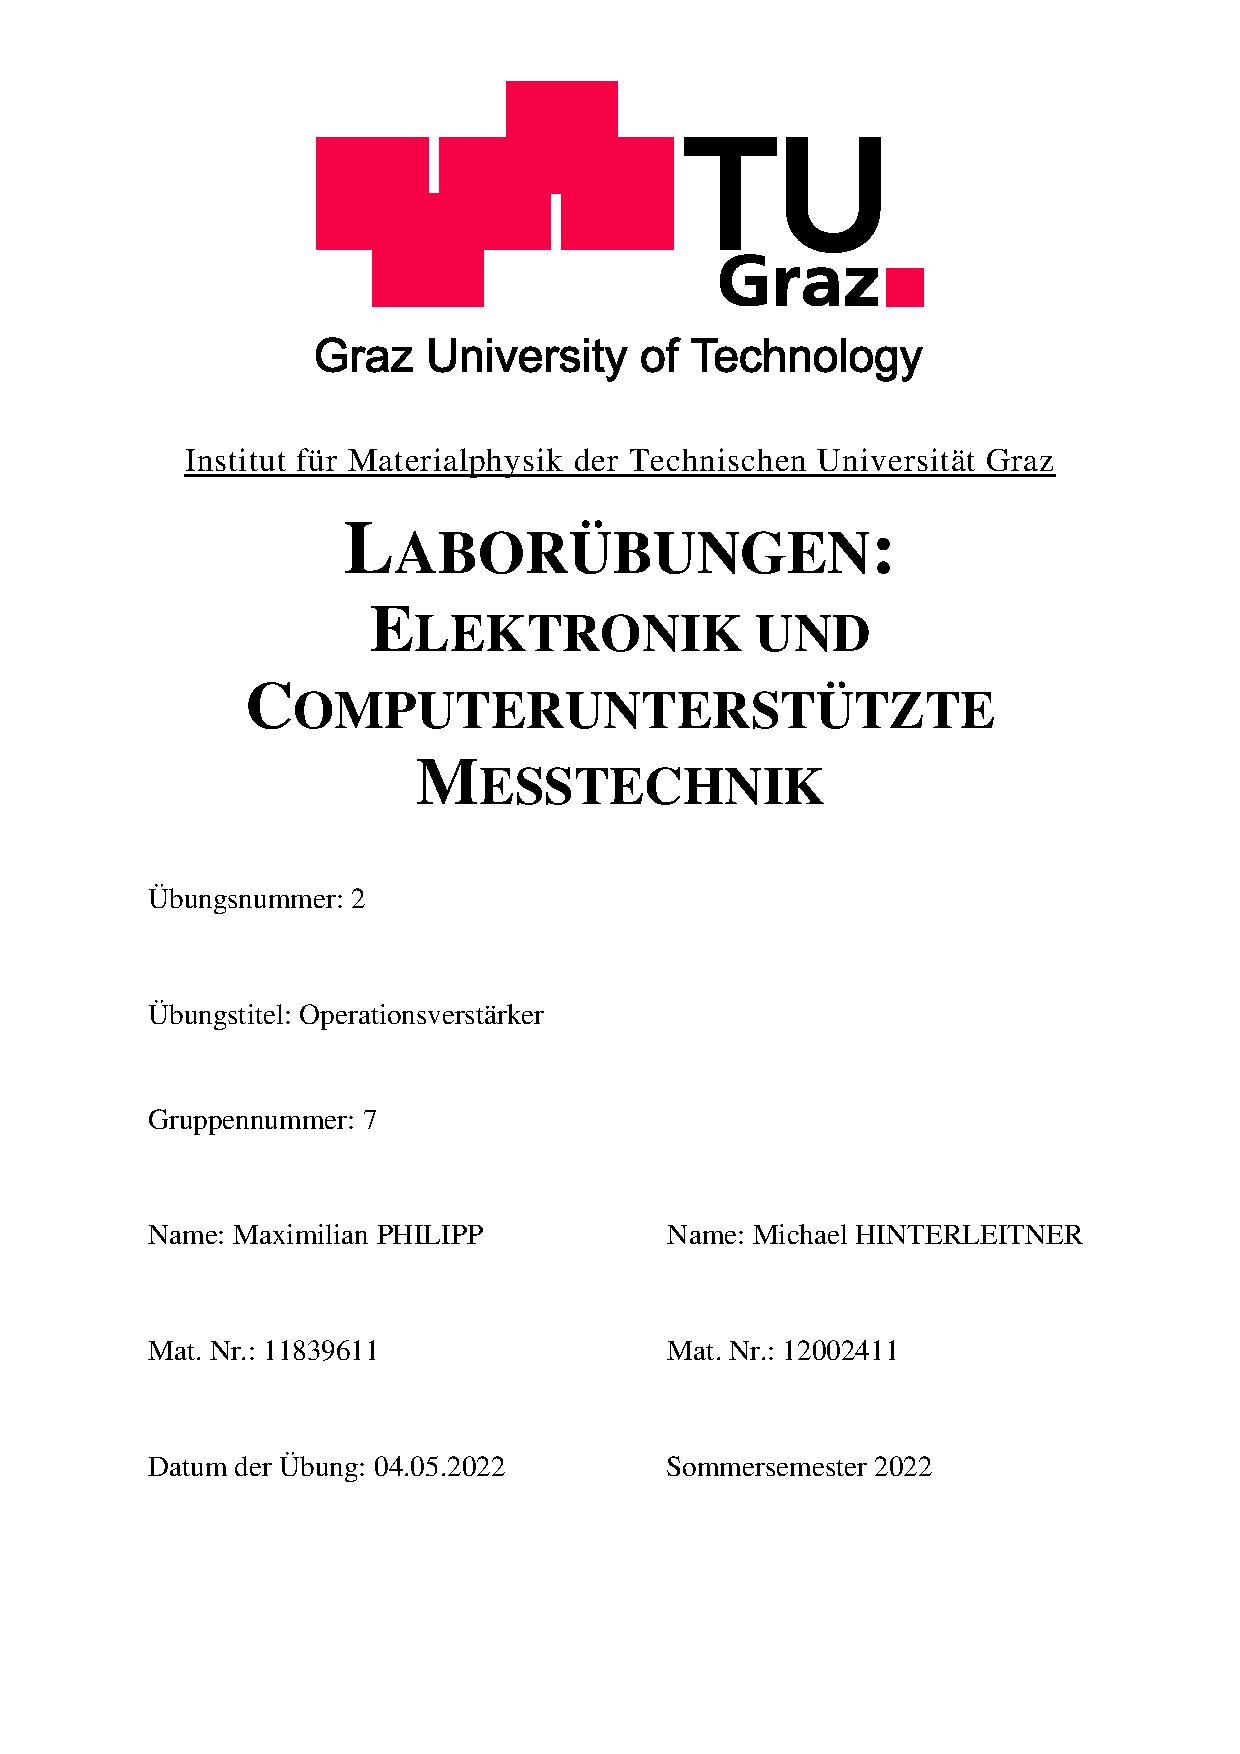
\includepdf{deckblatt2.pdf}
\tableofcontents
\newpage


%\section{Aufgabenstellung}\label{sec:Aufgabenstellung}

% Die nachfolgende Aufgabenstellung wurde von den Laborbetreuern bereitgestellt
% und beinhaltet sowohl Angaben zur Vorbereitung als auch zur praktischen
% Durchführung der Übung:

% zu 1: Aufgabenstellung Das vor der Übung verteilte Aufgabenblatt.
 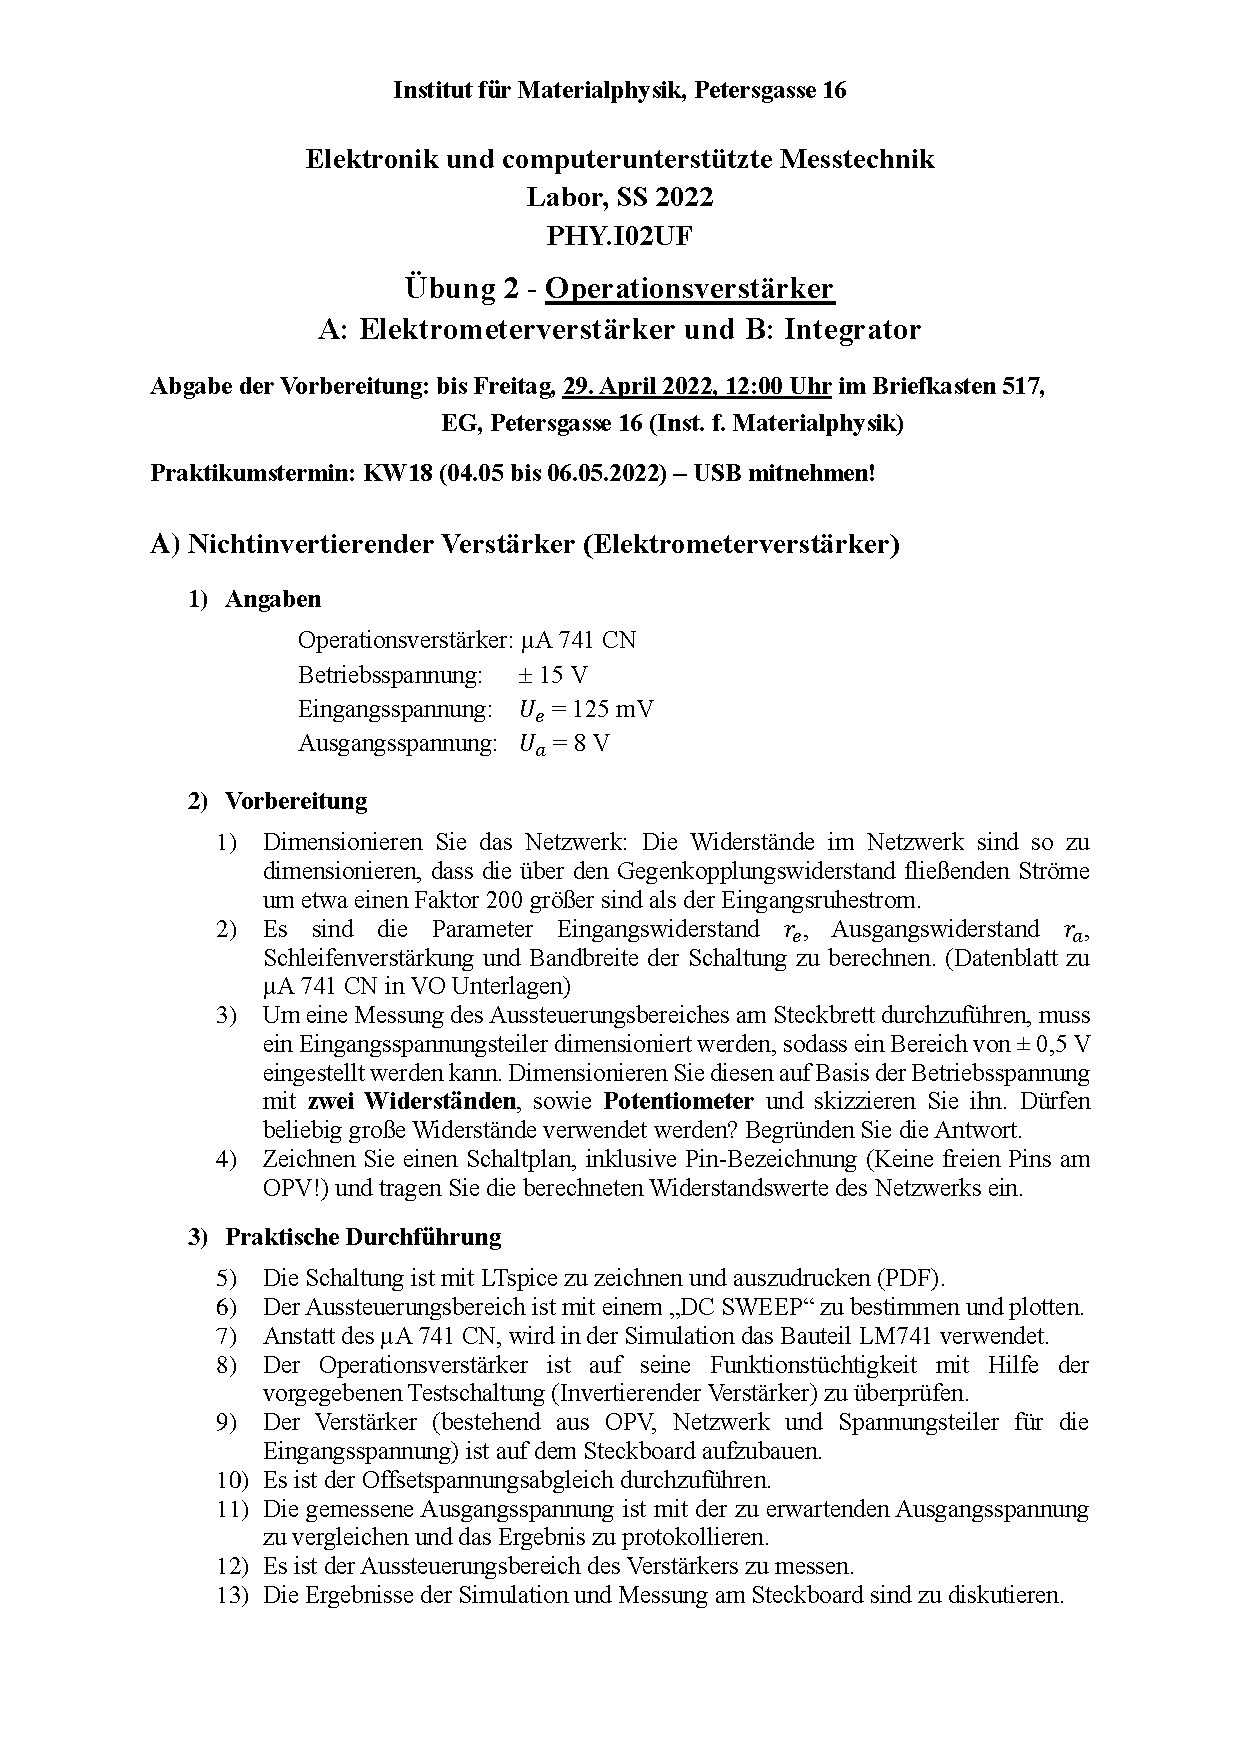
\includepdf[
     pages=-,  % all pages
     addtotoc={
         1, section, 1, Aufgabenstellung, sec:Aufgabenstellung
     }
 ]{angabe.pdf}

% zu 2: Vorbereitung Es sind beide Vorbereitungen dem Protokoll beizufügen.
% \section{Vorbereitung}\label{sec:Vorbereitung}
%Die folgende Vorbereitung wurde vor der Laborübung 
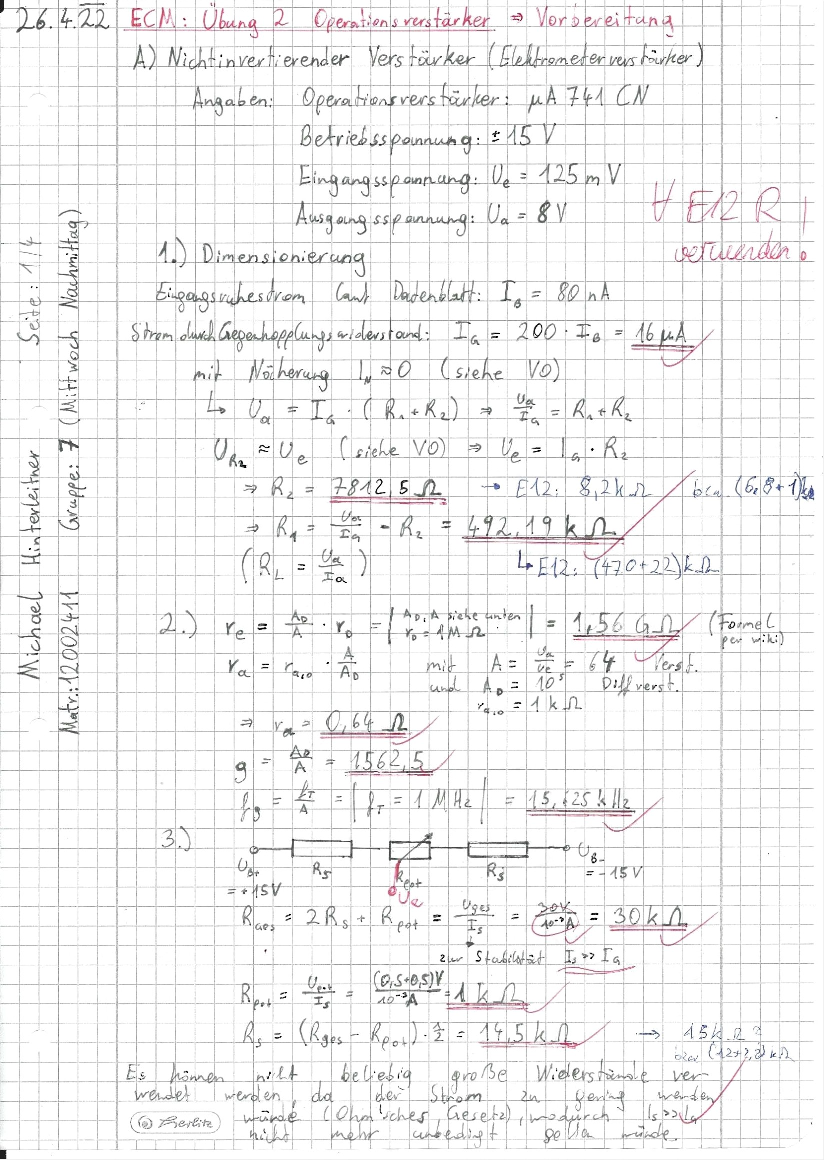
\includepdf[pages=-,
     addtotoc={
         1, section, 2, Vorbereitung, sec:Vorbereitung
     }]{./mh_vorbereitung_opv.pdf}
% 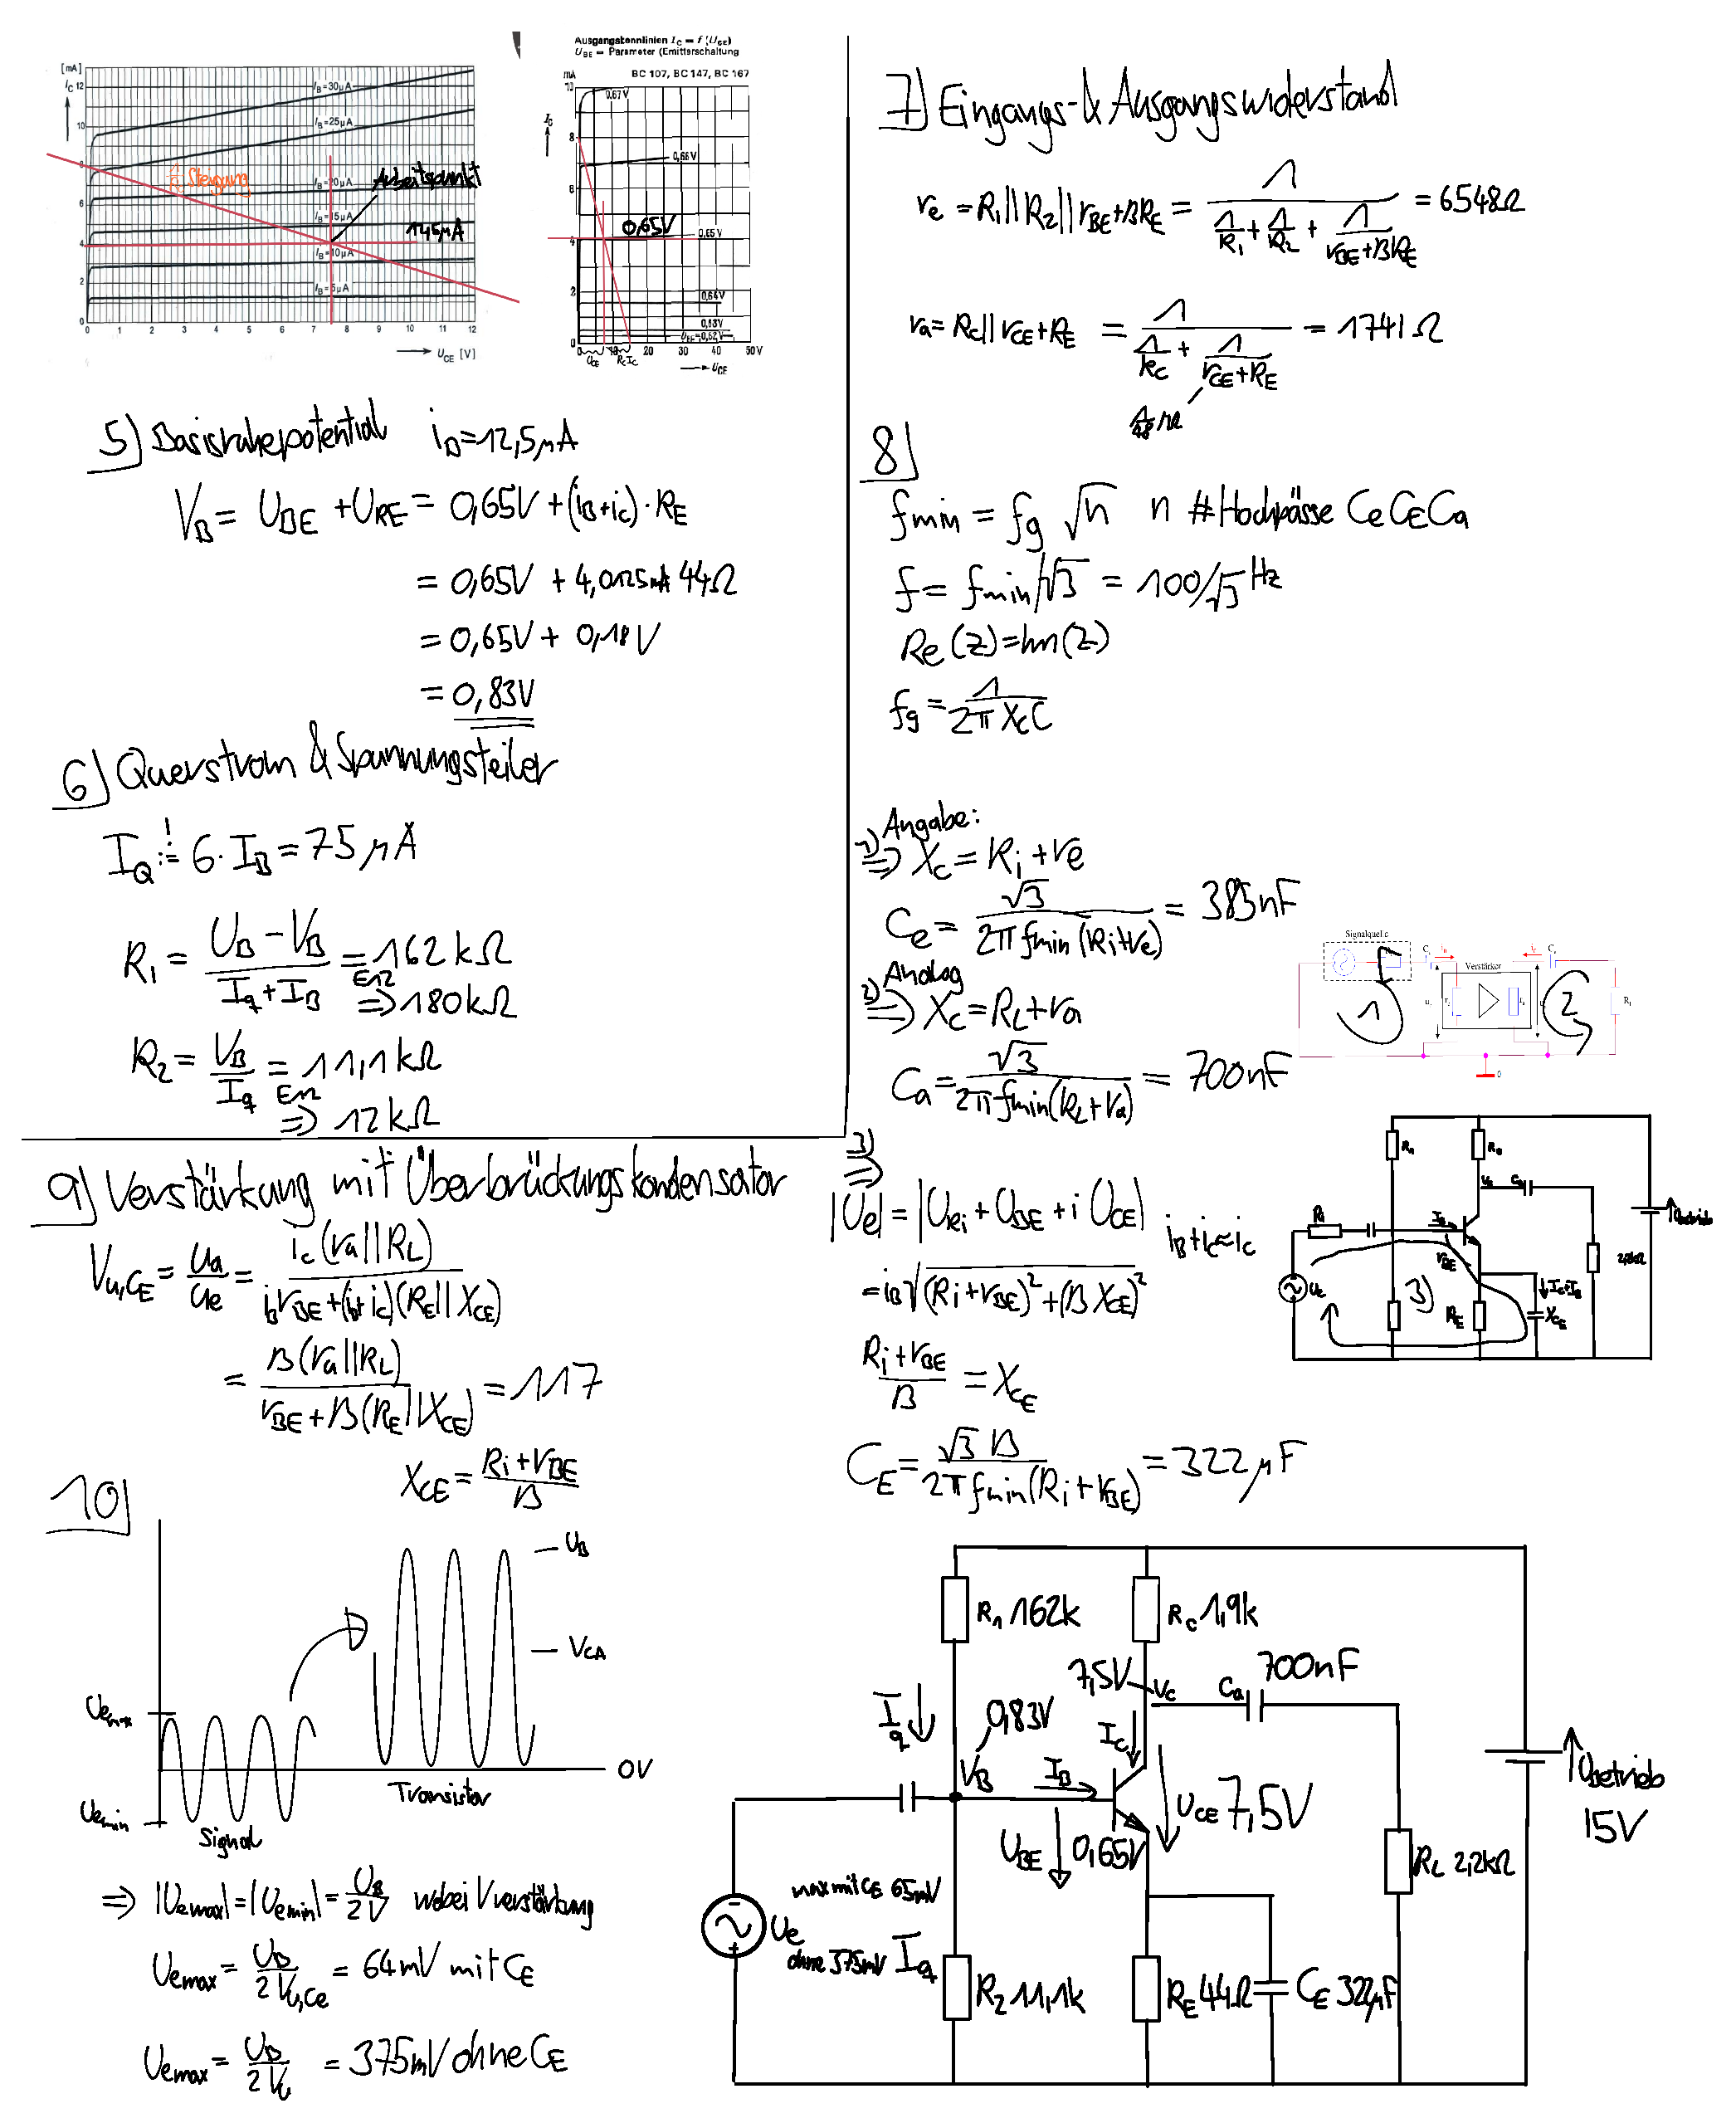
\includepdf[pages=-]{./figures/Transistor2.pdf}


% zu 3: Grundlagen In den Grundlagen sollen die später verwendeten Formeln
% stehen und kurz erklärt werden, dabei ist es nicht notwendig Formeln
% herzuleiten. Quellenangaben sind an dieser Stelle von Vorteil, weil Sie so
% schnell die betreffenden Stellen in Unterlagen finden. In den Rechnungen
% werden grundlegende Annahmen skizziert und begründet und dann mit diesen
% Annahmen, die für die Schaltungen notwendigen Werte berechnet. Dabei kann
% auch gleich auf die später wirklich verwendeten Werte Bezug genommen werden -
% wir verwenden bei den Widerständen zum Beispiel von den Normwert-Reihen die
% E12 und/oder E24 Serie (nach DIN 41426 bzw. IEC 63).
\section{Grundlagen}\label{sec:Grundlagen}
%in Grundlagen
Operationsverstärker (kurz 'OPV oder 'OpAmp') dienen grundlegend der Verstärkung von 
Gleichspannungen. Sie besitzen einen nicht-invertierenden, der meist mit einem 
Plus, und einen invertierenden Eingang, der mit einem Minus dargestellt wird. Zu 
beachten ist, dass die Verstärkung auf die Differenzspannung der beiden Eingänge 
wirkt. Je zwei zusätzliche Anschlüsse finden sich für die positive und negative 
Betriebsspannung und für den Offsetabgleich, damit bei keiner Eingangsspannung 
auch keine Ausgangsspannung auftritt - dieser wird also in einer externen 
Schaltung durchgeführt.

\begin{figure}[H]
    \centering
    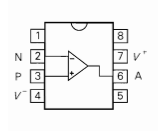
\includegraphics[width=6cm, height=6cm,keepaspectratio]{./figures/pics/pins.PNG}
    \caption{Schematische Darstellung der Pinbelegung eines klassischen Operationsverstärkers. Hierbei bezeichnet 2 den invertierenden, 3 den nicht-invertierenden Eingangskanal, 6 den Ausgang, 4 den Anschluss für die negative sowie 7 den Anschluss für die positive Betriebsspannung, 1 und 5 die Pins für den Offsetabgleich und 8 einen freien Pin.  \cite{tietze}}
    \label{fig:pin_anschl}
\end{figure}

In \autoref{fig:pin_anschl} sind die Pins eines Operationsverstärkers, wie er auch 
in der Laborübung verwendet wurde, zu sehen. Dabei ist zu beachten, dass jeder nicht 
belegte Pin auf Masse gelegt werden soll.

Es gibt vier grundlegende Arten der Verwendung von Operationsverstärkern, darunter
der nicht-invertierende Betrieb, bei dem das Eingangssignal nur auf den nicht-invertierenden 
Kanal gelegt wird und der invertierende auf Masse gelegt wird. Analog funktioniert der invertierende 
Modus, bei dem das Signal anstelle nun an den invertierenden Eingang gelegt wird, wodurch die Ausgangsspannung 
zusätzlich zur Verstärkung noch zum Eingangssignal invertiert wird. Beim Differenzbetrieb werden an 
beide Eingänge Signale angelegt und die Differenzspannung verstärkt. Im Falle des Gleichtaktbetriebs 
liegt das gleiche Eingangssignal an den beiden Eingängen an, wodurch es theoretisch keine Differenzspannung 
und Verstärkung geben sollte - in der Realität resultiert allerdings eine Verstärkung, die als 
Gleichtaktverstärkung bezeichnet wird.

Da der Operationsverstärker ohne zusätzliche Verkopplung sehr stark frequenzabhängig ist und 
nur eine geringe Bandbreite gewünscht verstärkt, wird eine Gegenkopplung vom Ausgang zum Eingang 
durchgeführt, wodurch die Verstärkung zwar abnimmt, die Bandbreite jedoch stark vergrößert wird. 
Die Bandbreite wird wie gewohnt durch die Grenzfrequenz charakterisiert, bei welcher die Verstärkung 
noch \SI{70}{\%} der maximalen beträgt. Wenn nun beispielsweise ein Kondensator in der Rückkopplung verbaut wird, 
handelt es sich um eine Integratorschaltung, die im zweiten Teil der Laborübung untersucht wird.

Die resultierende Verstärkung lässt sich gemäß \autoref{eq:ver} als Verhältnis der Ausgangs- $U_a$ zur Eingangsspannung $U_e$ berechnen.
\begin{equation}
	V=\frac{U_a}{U_e}
	\label{eq:ver}
\end{equation}


% zu 4: Versuchsdurchführung In diesem Punkt wird die Durchführung der
% einzelnen Aufgaben beschrieben. Im Simulationsteil ist die simulierte
% Schaltung mit allen Analyseparametern darzustellen. Im praktischen Teil sind
% die verwendete Geräte sowie die gemessenen Werte der verwendeten Bauteile
% anzugeben. Außerdem sind durchgeführte Funktionsüberprüfungen der Bauteile
% (Dioden, Transistor, etc.) anzuführen. Die Messergebnisse bzw. Oszillogramme
% sind mit Angabe der verwendeten Messgeräte anzugeben. Oszillogramme werden
% vom verwendeten Oszilloskop als Daten auf einen USB-Stick ausgegeben und
% können in das Protokoll aufgenommen werden. Das gleiche gilt für Schaltungen
% bzw. Ergebnissen von Simulationen. Es ist auf eine klare Darstellung der
% Messergebnisse und –auswertung zu achten (Tabellen, geeignete Grafiken). Die
% originalen, während des Versuchs angefertigten Aufzeichnungen sind dem
% Protokoll beizufügen. 
\section{Versuchsdurchführung}\label{sec:Versuchsdurchf}

\subsection{Elektrometerverstärker}

% 5) Die Schaltung ist mit LTspice zu zeichnen und auszudrucken (PDF).
\subsubsection{Simulation} \label{sec:Versuchsim}

% TODO text
Zur Simulation des Elektrometerverstärkers wird das Programm
\textit{LTSPICE} verwendet. Der Aufbau erfolgt analog zum skizzierten
Schaltplan \autoref{fig:sim_elektrometer_schaltung}. Hier wurde das gleiche
Bauteil wie im Kapitel \nameref{sec:Aufgabenstellung} verwendet der $\mu$A741.

\begin{figure}[H]
  \centering
  % TODO LTSPICE aufbau der Elektrometer
    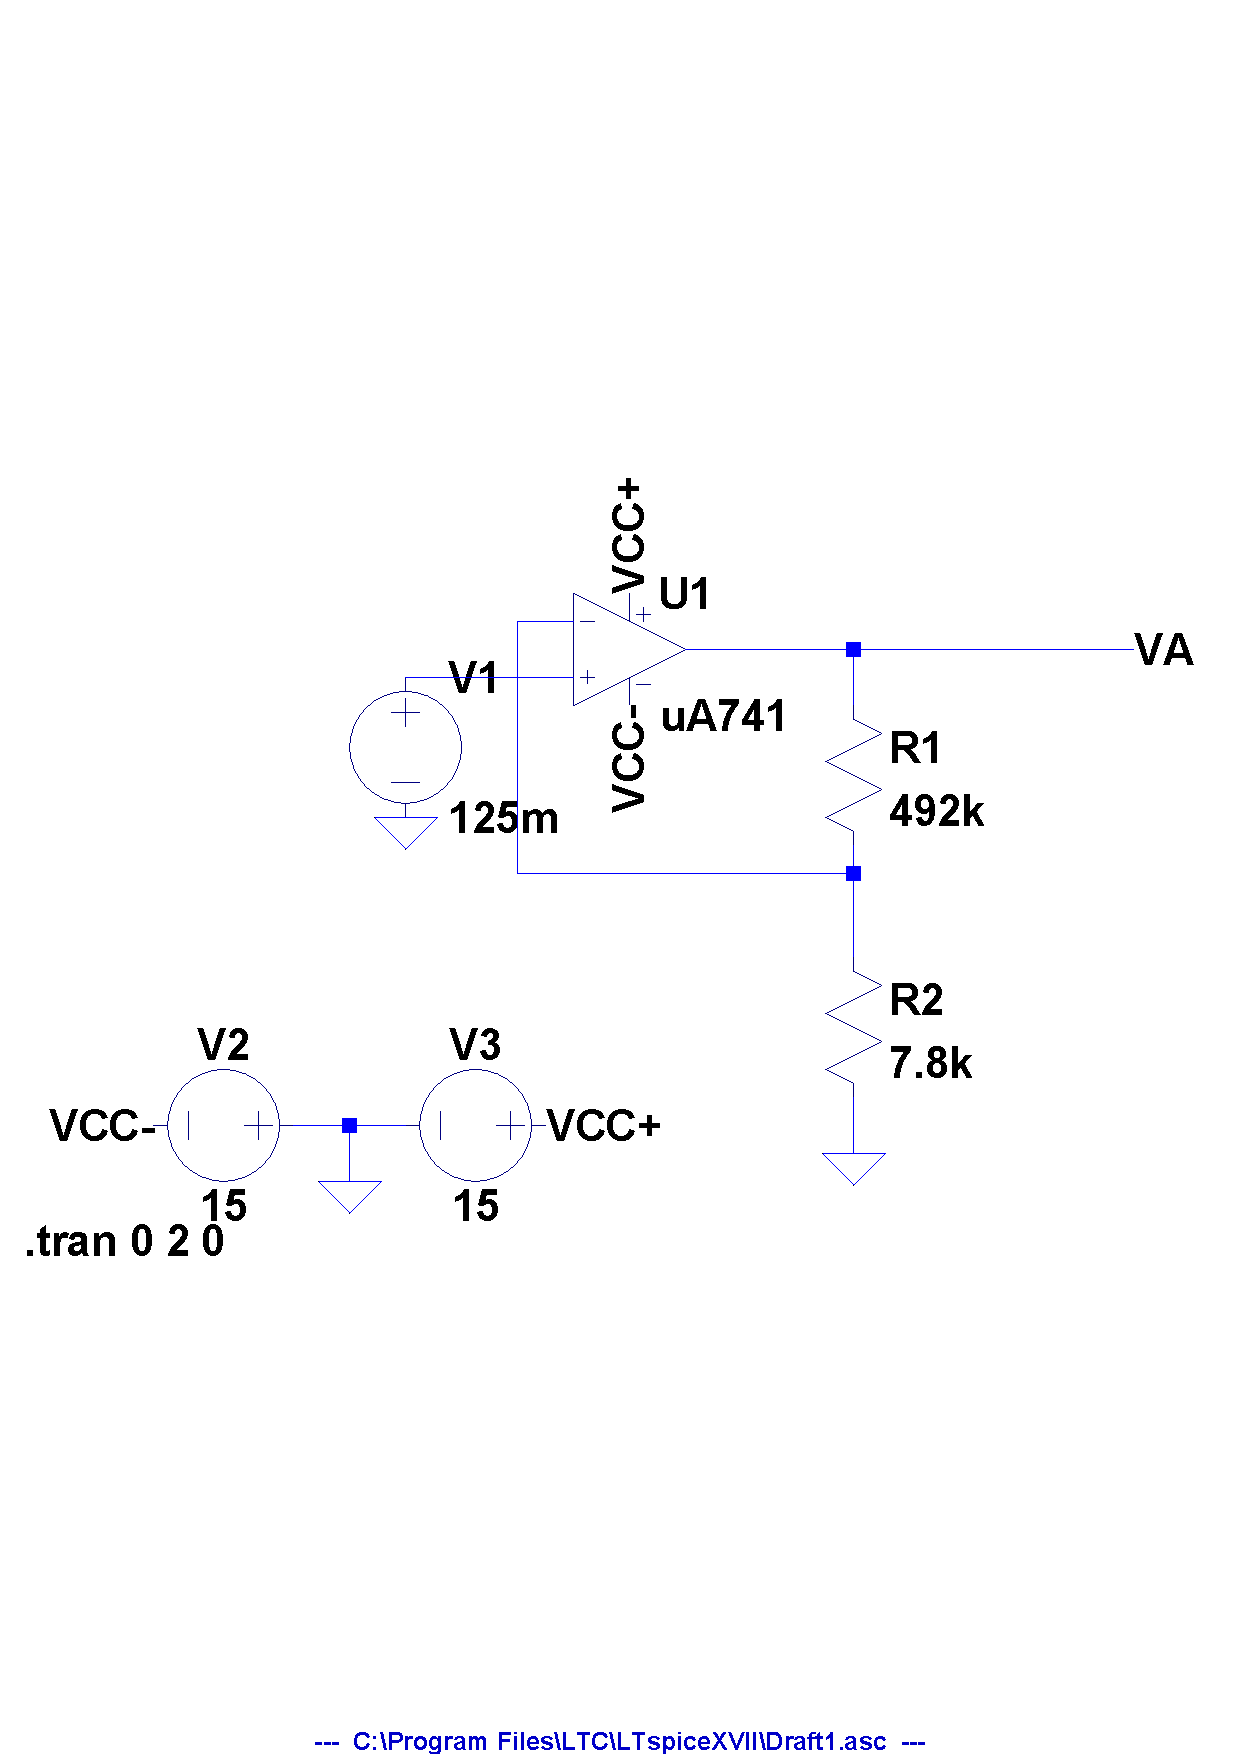
\includegraphics[width=0.95\textwidth]{./figures/elektrometer/sim/sim_schaltung.pdf}
  \caption{Dies ist die Elektrometerverstärkerschaltung aufgebaut in \textit{LTSPICE}}
  \label{fig:sim_elektrometer_schaltung}
\end{figure}


% 6) Der Aussteuerungsbereich ist mit einem „DC SWEEP“ zu bestimmen und plotten.
% 7) Anstatt des µA 741 CN, wird in der Simulation das Bauteil LM741 verwendet.
% NEIN fehler in der Angabe sollte UA741 bauteil sein
\paragraph{Untersuchung des Aussteuerungsbereichs} \label{sec:mess_aussteuerungsbereich}


\begin{figure}[H]
  \centering
  % TODO LTSPICE dc sweep von ausgangsspannung 
    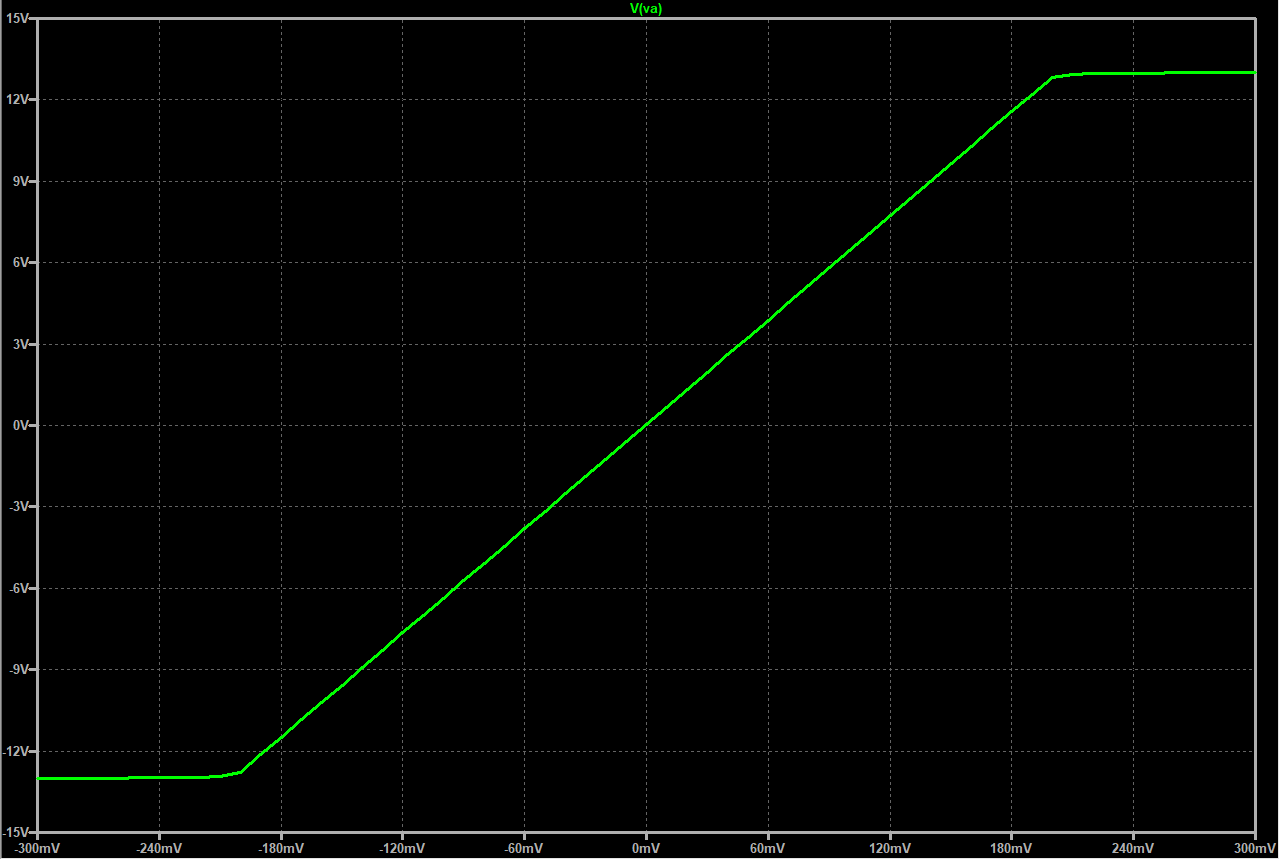
\includegraphics[width=0.95\textwidth]{./figures/elektrometer/sim/aus_sweep.png}
  % TODO check spice directive
  \caption{Die Schaltung aus \autoref{fig:sim_elektrometer_schaltung} wurde auf
  den Aussteuerungsbereich untersucht in dem ein DC-Sweep gemacht wurde. Die
  Simulation SPICE-Directive ist \texttt{.dc V1 -0.3 0.3 0.01}}
  \label{fig:sim_elektrometer_dcsweep}
\end{figure}

\subsubsection{Steckbrett} \label{sec:elektrometer_steckbrett}
% TODO neuer text
% Zunächst wird die Schaltung allerdings ohne Überbrückungskondensator, wie sie
% in  \autoref{fig:schaltungohnekond} zu sehen ist, verwendet. Nachdem
% alle Parameter gemäß den Angaben in der Simulation und insbesondere der
% Arbeitspunkt entsprechend dem theoretisch errechneten Wert eingestellt wurden
% (ca. \SI{7.5}{\volt}), wurden die Eingangs- und Ausgangsspannung über der Zeit in
% einem Plot, durch Messung dieser Größen für einen geeigneten Zeitabschnitt
% (siehe  \autoref{fig:schaltungohnekond} im unteren Bildbereich),
% dargestellt. 

\paragraph{Testschaltung}
% 8) Der Operationsverstärker ist auf seine Funktionstüchtigkeit mit Hilfe der
% vorgegebenen Testschaltung (Invertierender Verstärker) zu überprüfen.
Zur Untersuchung der Funktionstüchtigkeit des OPVs wurde die im Lab vorhandene
Testschaltung, siehe \autoref{fig:testschaltung}, verwendet. 

\begin{figure}[H]
  \centering
  % TODO grafik einfuegen
    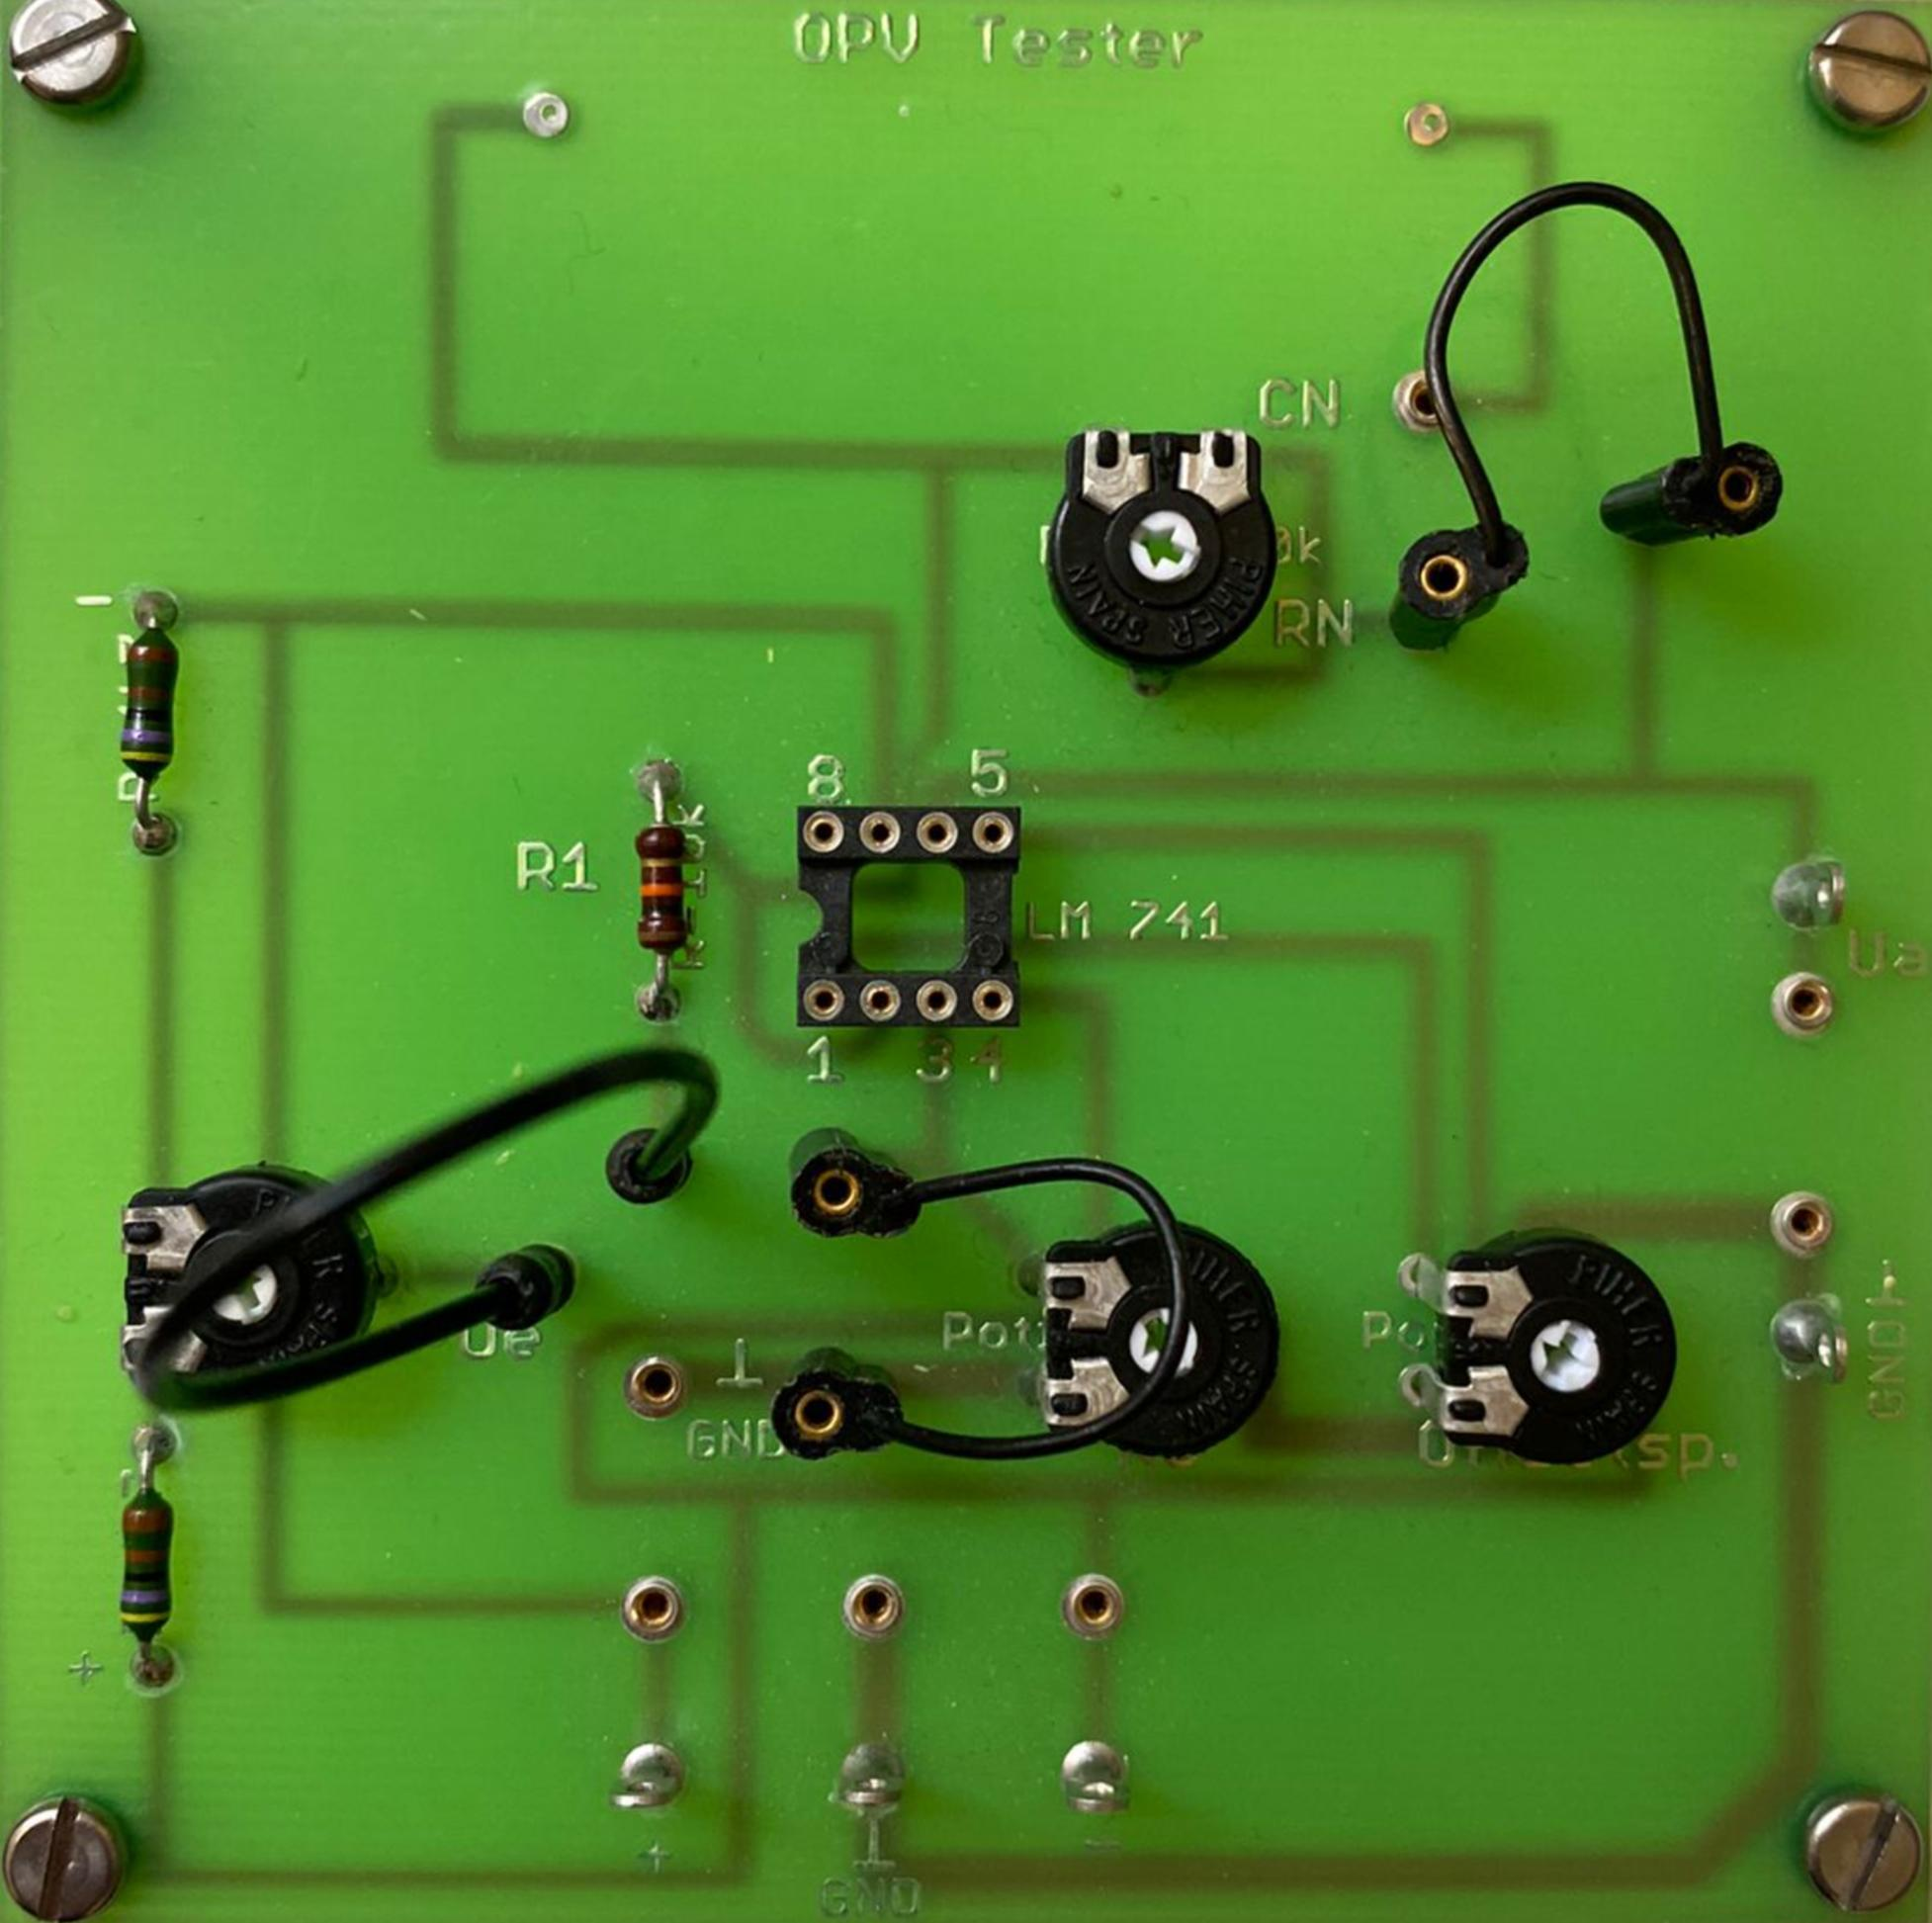
\includegraphics[width=0.95\textwidth]{./figures/testschaltung.jpeg}
  \caption{Das vorhandene Testbrett. Invertierender Verstärker}
  \label{fig:testschaltung}
\end{figure}

Diese Schaltung wurde verwendet um zu überprüfen ob der OPVs noch immer die
gewünschten Eigenschaften für positive und negative Verstärkung aufweißt. Dies
wurde durch das Variieren des Potentiometers (und somit das Variieren der
Eingangspannung) und dem Messen der Ausgangsspannung überprüft.

% 9) Der Verstärker (bestehend aus OPV, Netzwerk und Spannungsteiler für die
% Eingangsspannung) ist auf dem Steckboard aufzubauen.
\paragraph{Aufbau}

\begin{figure}[H]
  \centering
  % TODO grafik einfuegen
    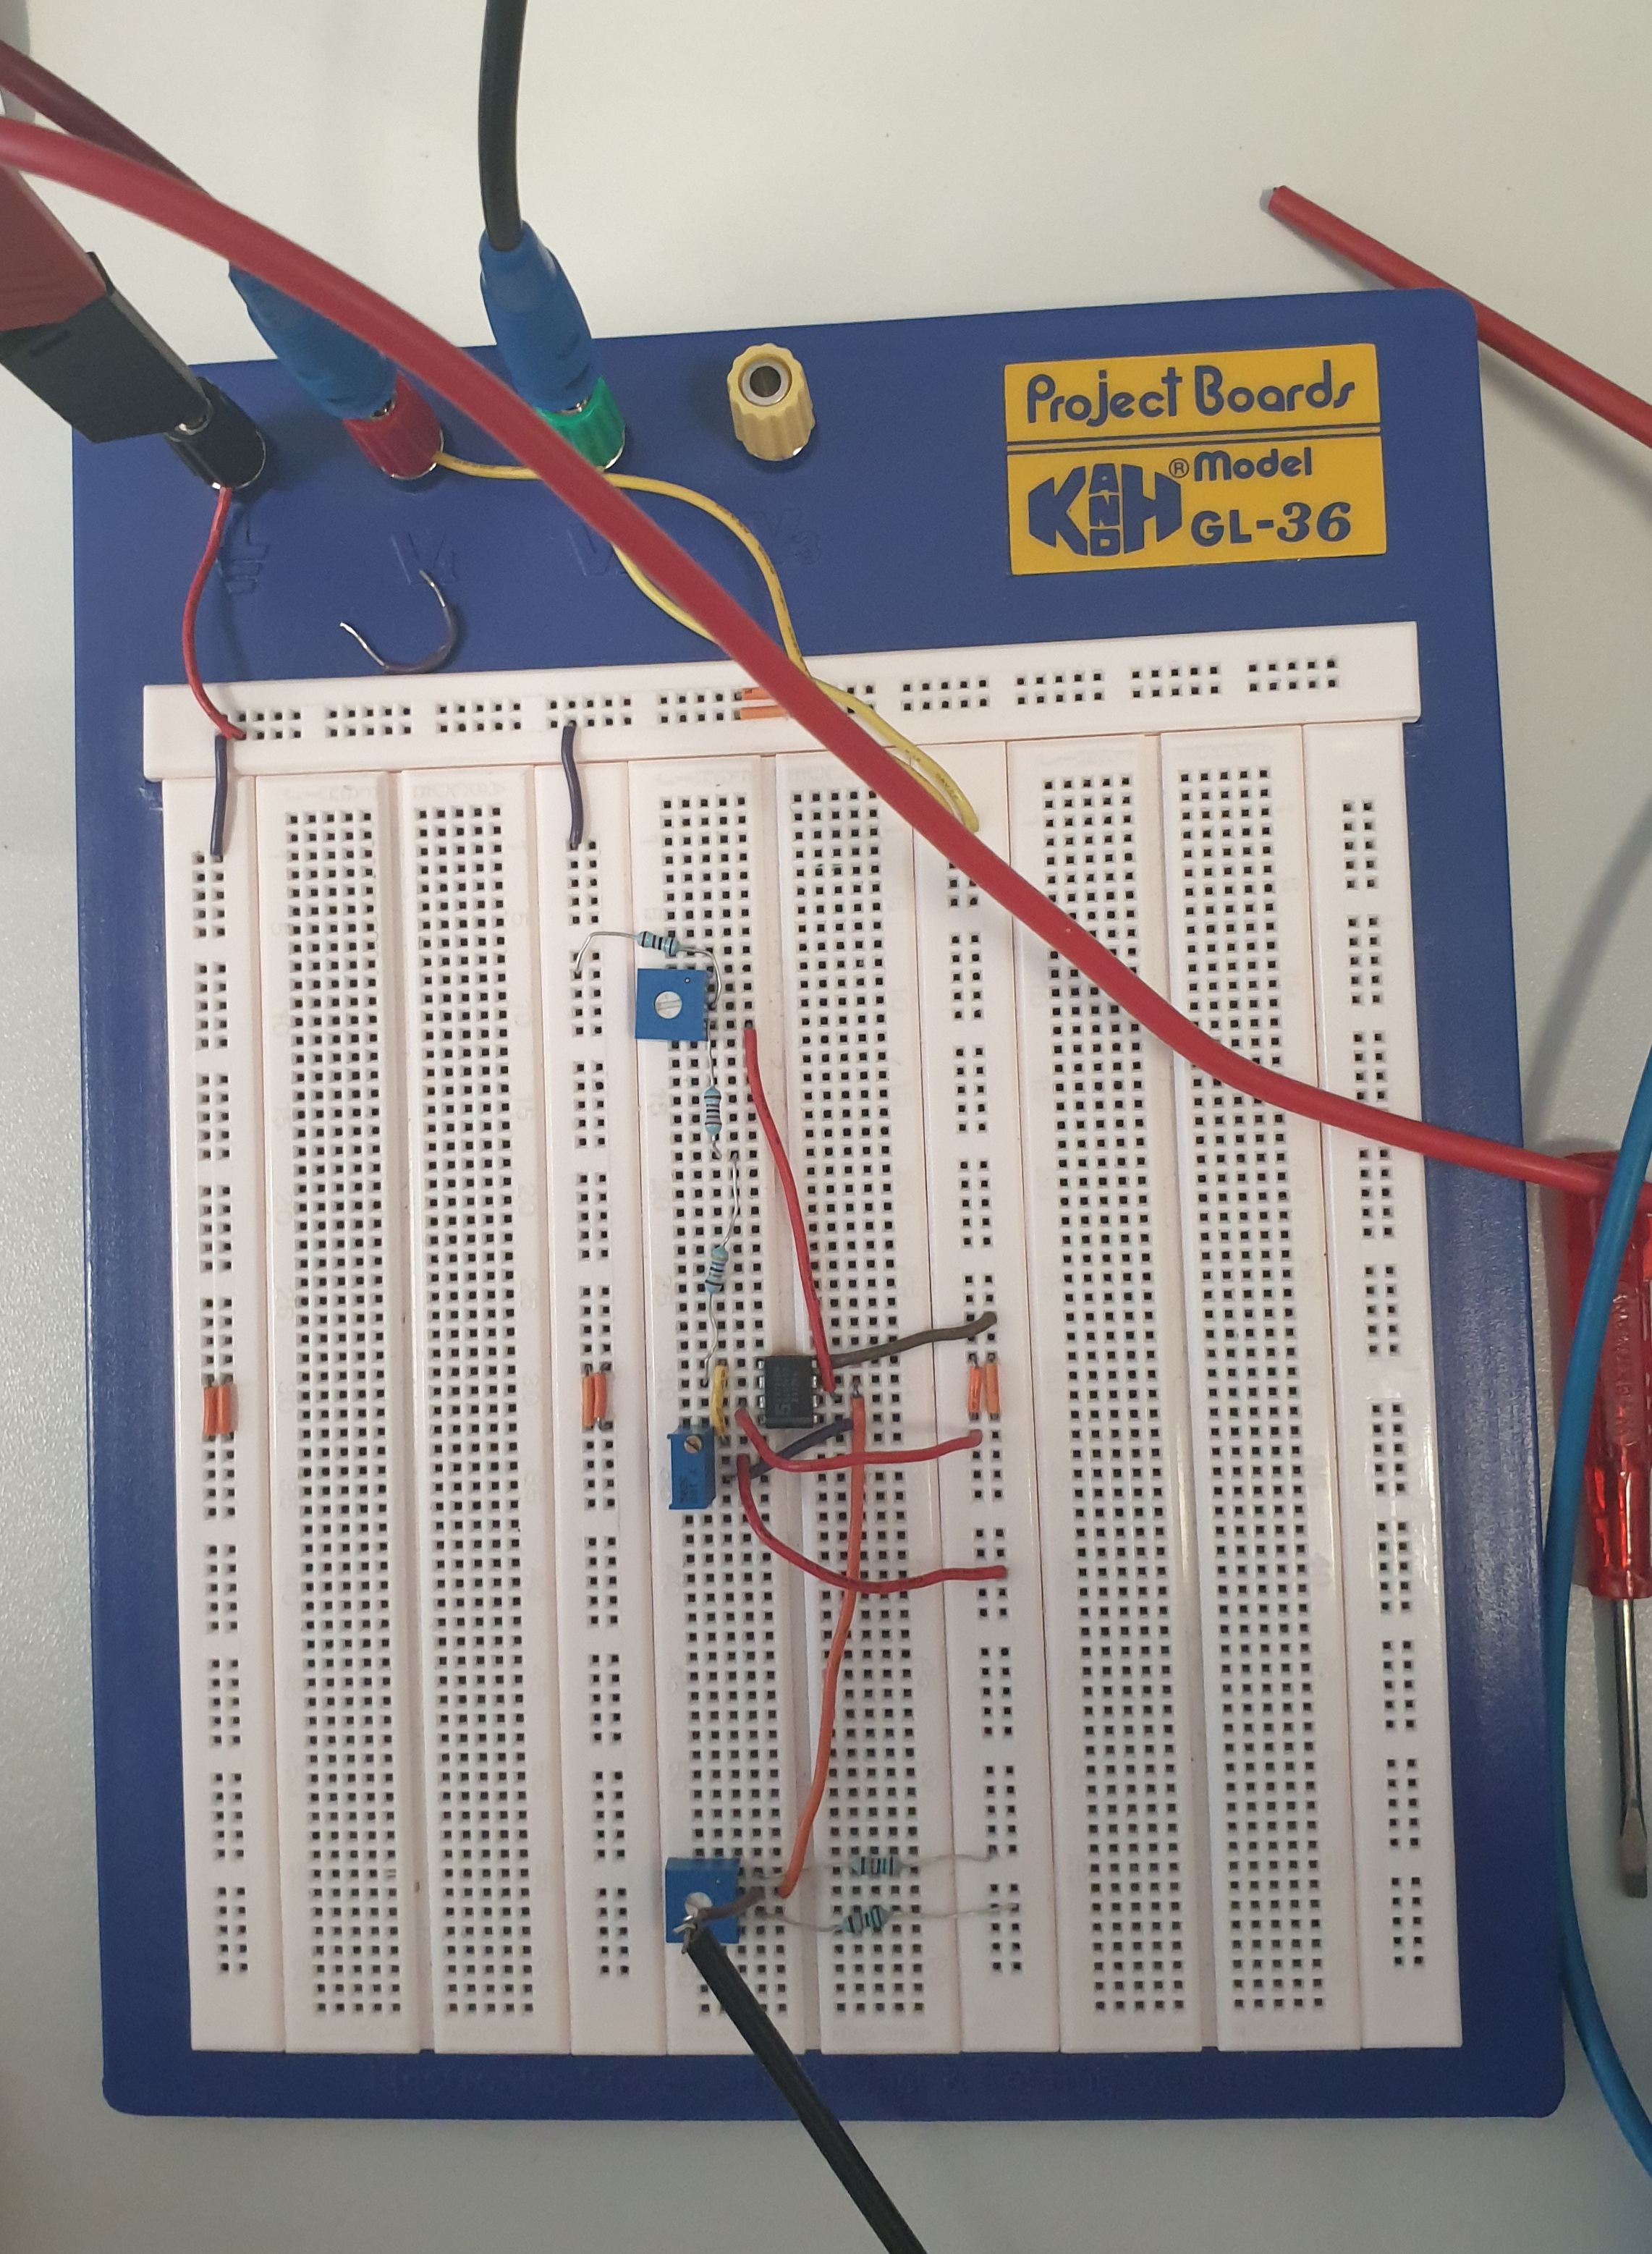
\includegraphics[width=0.95\textwidth]{./figures/elektrometer/steckbrett.png}
  \caption{Elektrometerverstärker Aufbau am Steckbrett der Schaltung von
  \autoref{fig:sim_elektrometer_schaltung}}
  \label{fig:ver_elektromete_aufbau}
\end{figure}

% 10) Es ist der Offsetspannungsabgleich durchzuführen.
\paragraph{Offsetabgleich}\label{sec:offsetabgleich}
Um den Offestspannungableich durchführen zu können ist zuerst mal ein
Impdanzwandel aufgebaut worden, wodurch das Abgleichen sich zum Abstimmen
der Eingangsspannug zur Ausgangsspannung vereinfachte. Dies wurde durch einen
extern Beschalteten Potentiometer bewerkstelligt, welcher die Rolle eines
Spannungteilers spielte. Der Offsetabgleich wurde bei einer Spannung von
\SI{125.4}{\milli\volt} gemacht.

% 11) Die gemessene Ausgangsspannung ist mit der zu erwartenden Ausgangsspannung
% zu vergleichen und das Ergebnis zu protokollieren.
\paragraph{Beschaltung als Elektrometerverstärker}
Nun wurde die Rückkopplung durch einen Spannungsteiler, wie in
\autoref{fig:sim_elektrometer_schaltung} ersichtlich, statt dem Kurzschluss vom
Ausgang zum invertierenden Eingang eingebaut. Zunächst gab es Probleme mit dem
Aufnehmen der Verstärkung, da der Ground einen Wackelkontakt bekommen hat,
welcher durch leichtes drehen des Anschlusses repariert werden konnte.
Nun konnte die $U_a$ und $U_e$ des Elektrometerverstärker gemessen werden. Dies
wurde mittels zwei Multimeter bewerkstelligt, indem wie in
\autoref{fig:sim_elektrometer_schaltung} ersichtlich über die Spannungsquelle
$V1$ und von $VA$ zu Masse gemessen wurde.

\begin{equation}
  U_a = \SI{8.03}{\volt} \quad @\, U_e = \SI{125.0}{\milli\volt}
  \label{eq:messwert_elektro_ausgang_eingang}
\end{equation}

% 12) Es ist der Aussteuerungsbereich des Verstärkers zu messen.
\paragraph{Untersuchung des Aussteuerungsbereichs} \label{sec:Versuchohnekond}


\begin{table}[H]
  \caption{Gemessene Ausgangs- und Eingangspannungen der Elektrometerschaltung
  zur Untersuchung des Aussteuerungsbereich\\
  $U_a \dots$ Ausgangsspannung \\
  $U_e \dots$ Eingangspannung \\
  }
  \label{tab:mess_elektro_aussteurerung}
  \centering
    \begin{tabular}[c]{S|S}
      {$U_e$ / \si{\milli\volt}} & {$U_a$ / \si{\volt}} \\
      0.0 & 0.0365 \\
      63.2 & 4.082 \\
      121.5 & 7.81 \\
      180.7 & 11.6 \\
      200.4 & 12.86 \\
      225.2 & 13.98 \\
      244.8 & 13.98 \\
      -62.8 & -3.987 \\
      -117.8 & -7.46 \\
      -176.2 & -11.24 \\
      -233.6 & -13.00 \\
      -290.6 & -13.35 \\
      -298.6 & -13.40 \\
      -340.1 & -13.49 \\
    \end{tabular}
\end{table}


% 13) Die Ergebnisse der Simulation und Messung am Steckboard sind zu diskutieren.

\subsection{Integrator}
% 1) Der Umkehrintegrator ist mit LTspice zu zeichnen und als Abbildung zu speichern.

\subsubsection{Simulation}
Zur Simulation des Elektrometerverstärkers wird das Programm
\textit{LTSPICE} verwendet. Der Aufbau erfolgt analog zum skizzierten
Schaltplan \autoref{fig:sim_integrator_schaltung}. 

\begin{figure}[H]
  \centering
  % TODO LTSPICE aufbau der Elektrometer
    % 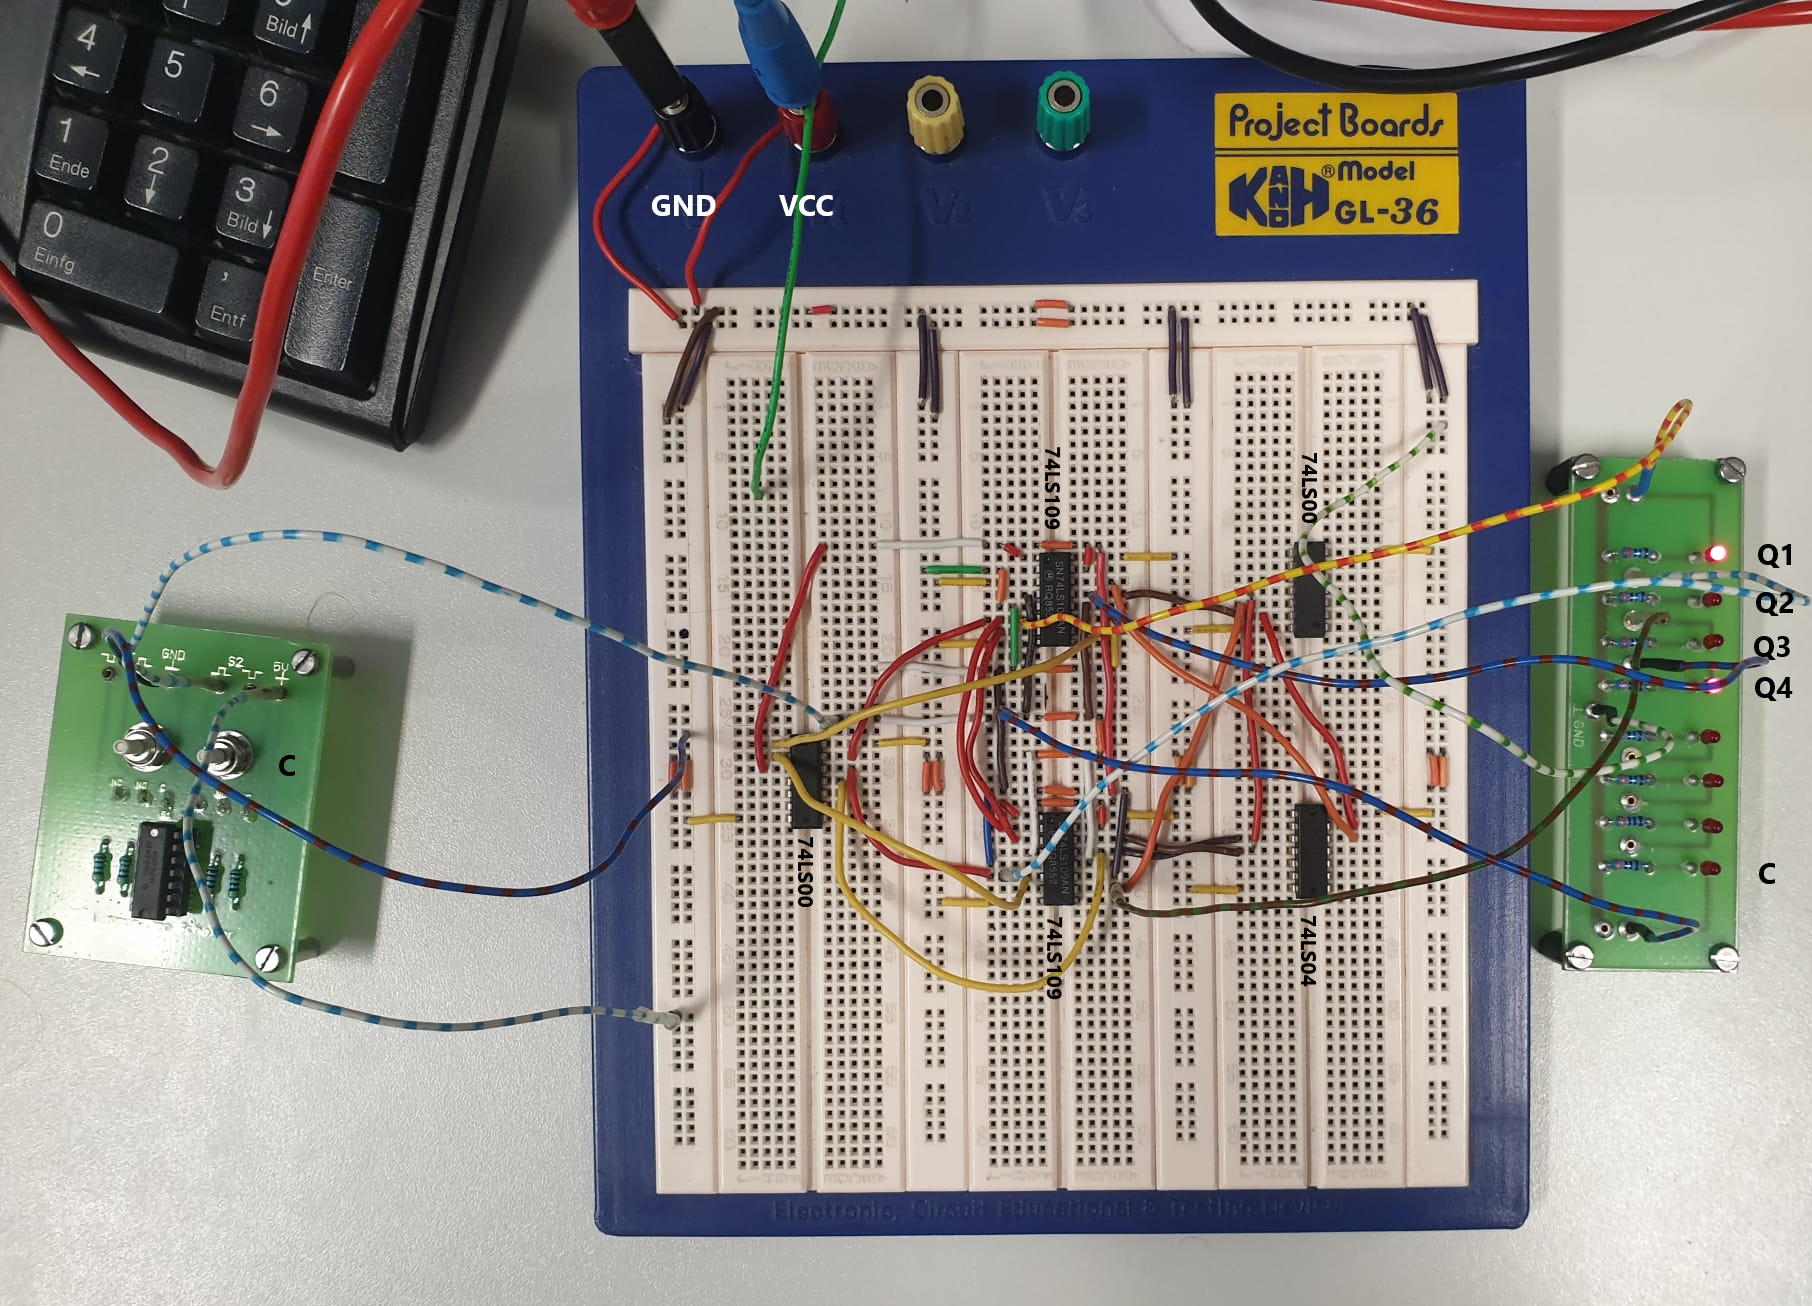
\includegraphics[width=0.95\textwidth]{./figures/integrator/aufbau.png}
  \caption{Dies ist die Integratorschaltung aufgebaut in \textit{LTSPICE}}
  \label{fig:sim_integrator_schaltung}
\end{figure}

% 2) Die Integrationsdauer der Schaltung ist mit einer konstanten Spannungsquelle zu
% simulieren. Die Ergebnisse sind mit der Vorbereitung zu vergleichen.
\paragraph{Integrationszeit}
Um die Integrationszeit zu bestimmen wurde eine Transiente-Analyse durchgeführt.

% TODO text

\begin{figure}[H]
  \centering
  % TODO LTSPICE trans anal von lade vorgang 
    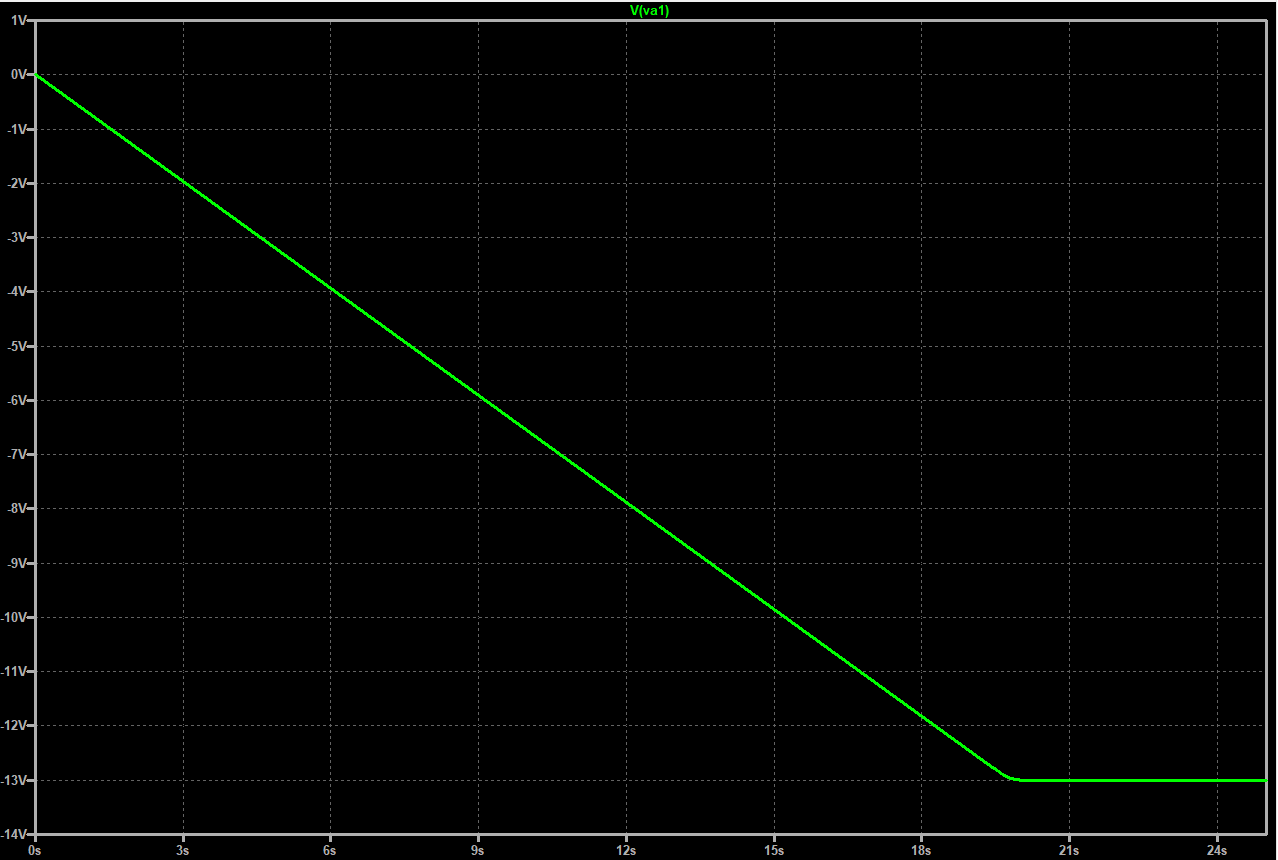
\includegraphics[width=0.95\textwidth]{./figures/integrator/sim/umkehr_int/dauer_aussteu.png}
  % TODO check spice directive
  \caption{Die Schaltung aus \autoref{fig:sim_integrator_schaltung} wurde auf
  die Integrationszeit untersucht in dem eine Transiente-Analyse vom
  Ladevorgang gemacht wurde. Die Simulation SPICE-Directive ist \texttt{.tran 0 25 0} 
  bei einer Eingangspannung $U_e$ von \SI{100}{\milli\volt}.}
  \label{fig:sim_integrator_integrationszeit}
\end{figure}

\subsubsection{Steckbrett}
% 3) Der OPV ist auf die Funktionstüchtigkeit zu prüfen. (siehe Aufgabe A, Punkt 8)
% 5) Es ist der Offsetspannungsabgleich durchzuführen.
Wie in \autoref{sec:offsetabgleich} erklärt, wurde nochmals mit der
Impdanzwandlerschaltung die Funktionstüchtigkeit überprüft. Ebenfalls wurde
gleich die Offsetabgleich nochmals überprüft. Jedoch musste dieser nicht
angepasst werden, da noch immer alles kalibriert war.

% 4) Der Umkehrintegrator (bestehend aus OPV, Netzwerk und Spannungsteiler) ist auf
% dem Steckboard aufzubauen.
% 6) Die aufgebaute Schaltung ist in Betrieb zu nehmen und die Integrationszeit zu
% protokollieren (Stoppuhr). Die Messung ist fünfmal zu wiederholen.
\paragraph{Integrationszeit}

Nun wurde die charakteristische Ingetrationszeit der Schaltung bestimmt. Indem
zuerst der Kondensator, bis das Multimeter am Ausgang \SI{0}{\mV} anzeigte,
entladen wurde und danach ist die Zeit des Ladens, die die Schaltung brauchte
um die geforderte Spannung von \SI{10}{\volt} am Ausgang zu haben, gemessen.
Dies wurde 6 mal wiederholt um eine Mittelung der Messergebnisse durchführen zu
können.

\begin{table}
  \caption{Messungen der Integrationszeit der realen Schaltung aus
  \autoref{fig:sim_integrator_schaltung}, wobei $T$ die Ladezeit bis am Ausgang
  \SI{10}{\volt} anliegt. Bei einem Ladespannung \SI{91.8}{\milli\volt}, einem
  Widerstand von \SI{21.9}{\kilo\ohm} und einer Kapazität von
  \SI{6.8}{\micro\farad} }
  \label{tab:messungen_integration}
  \centering
  \begin{tabular}[c]{S}
    {$T$ / \si{\second}} \\
    17.20 \\
    16.42 \\
    16.90 \\
    16.89 \\
    17.32 \\
    17.21 \\
  \end{tabular}
\end{table}


% 7) Die Schaltung (und Simulation) ist mit verschiedenen Spannungsquellen (Sinus,
% Rechteck, Dreieck) zu testen. Protokollieren und vergleichen Sie die Ergebnisse.
% Nutzen Sie dazu Oszilloskop und Frequenzgenerator.

\paragraph{Untersuchung Verschiedene Eingangssignale}
Nun wurde die Integrationsfähigkeit der Schaltung durch Einspeisen
verschiedener Eingangssignal qualitative untersucht.
 
\begin{figure}[H]
  \centering
    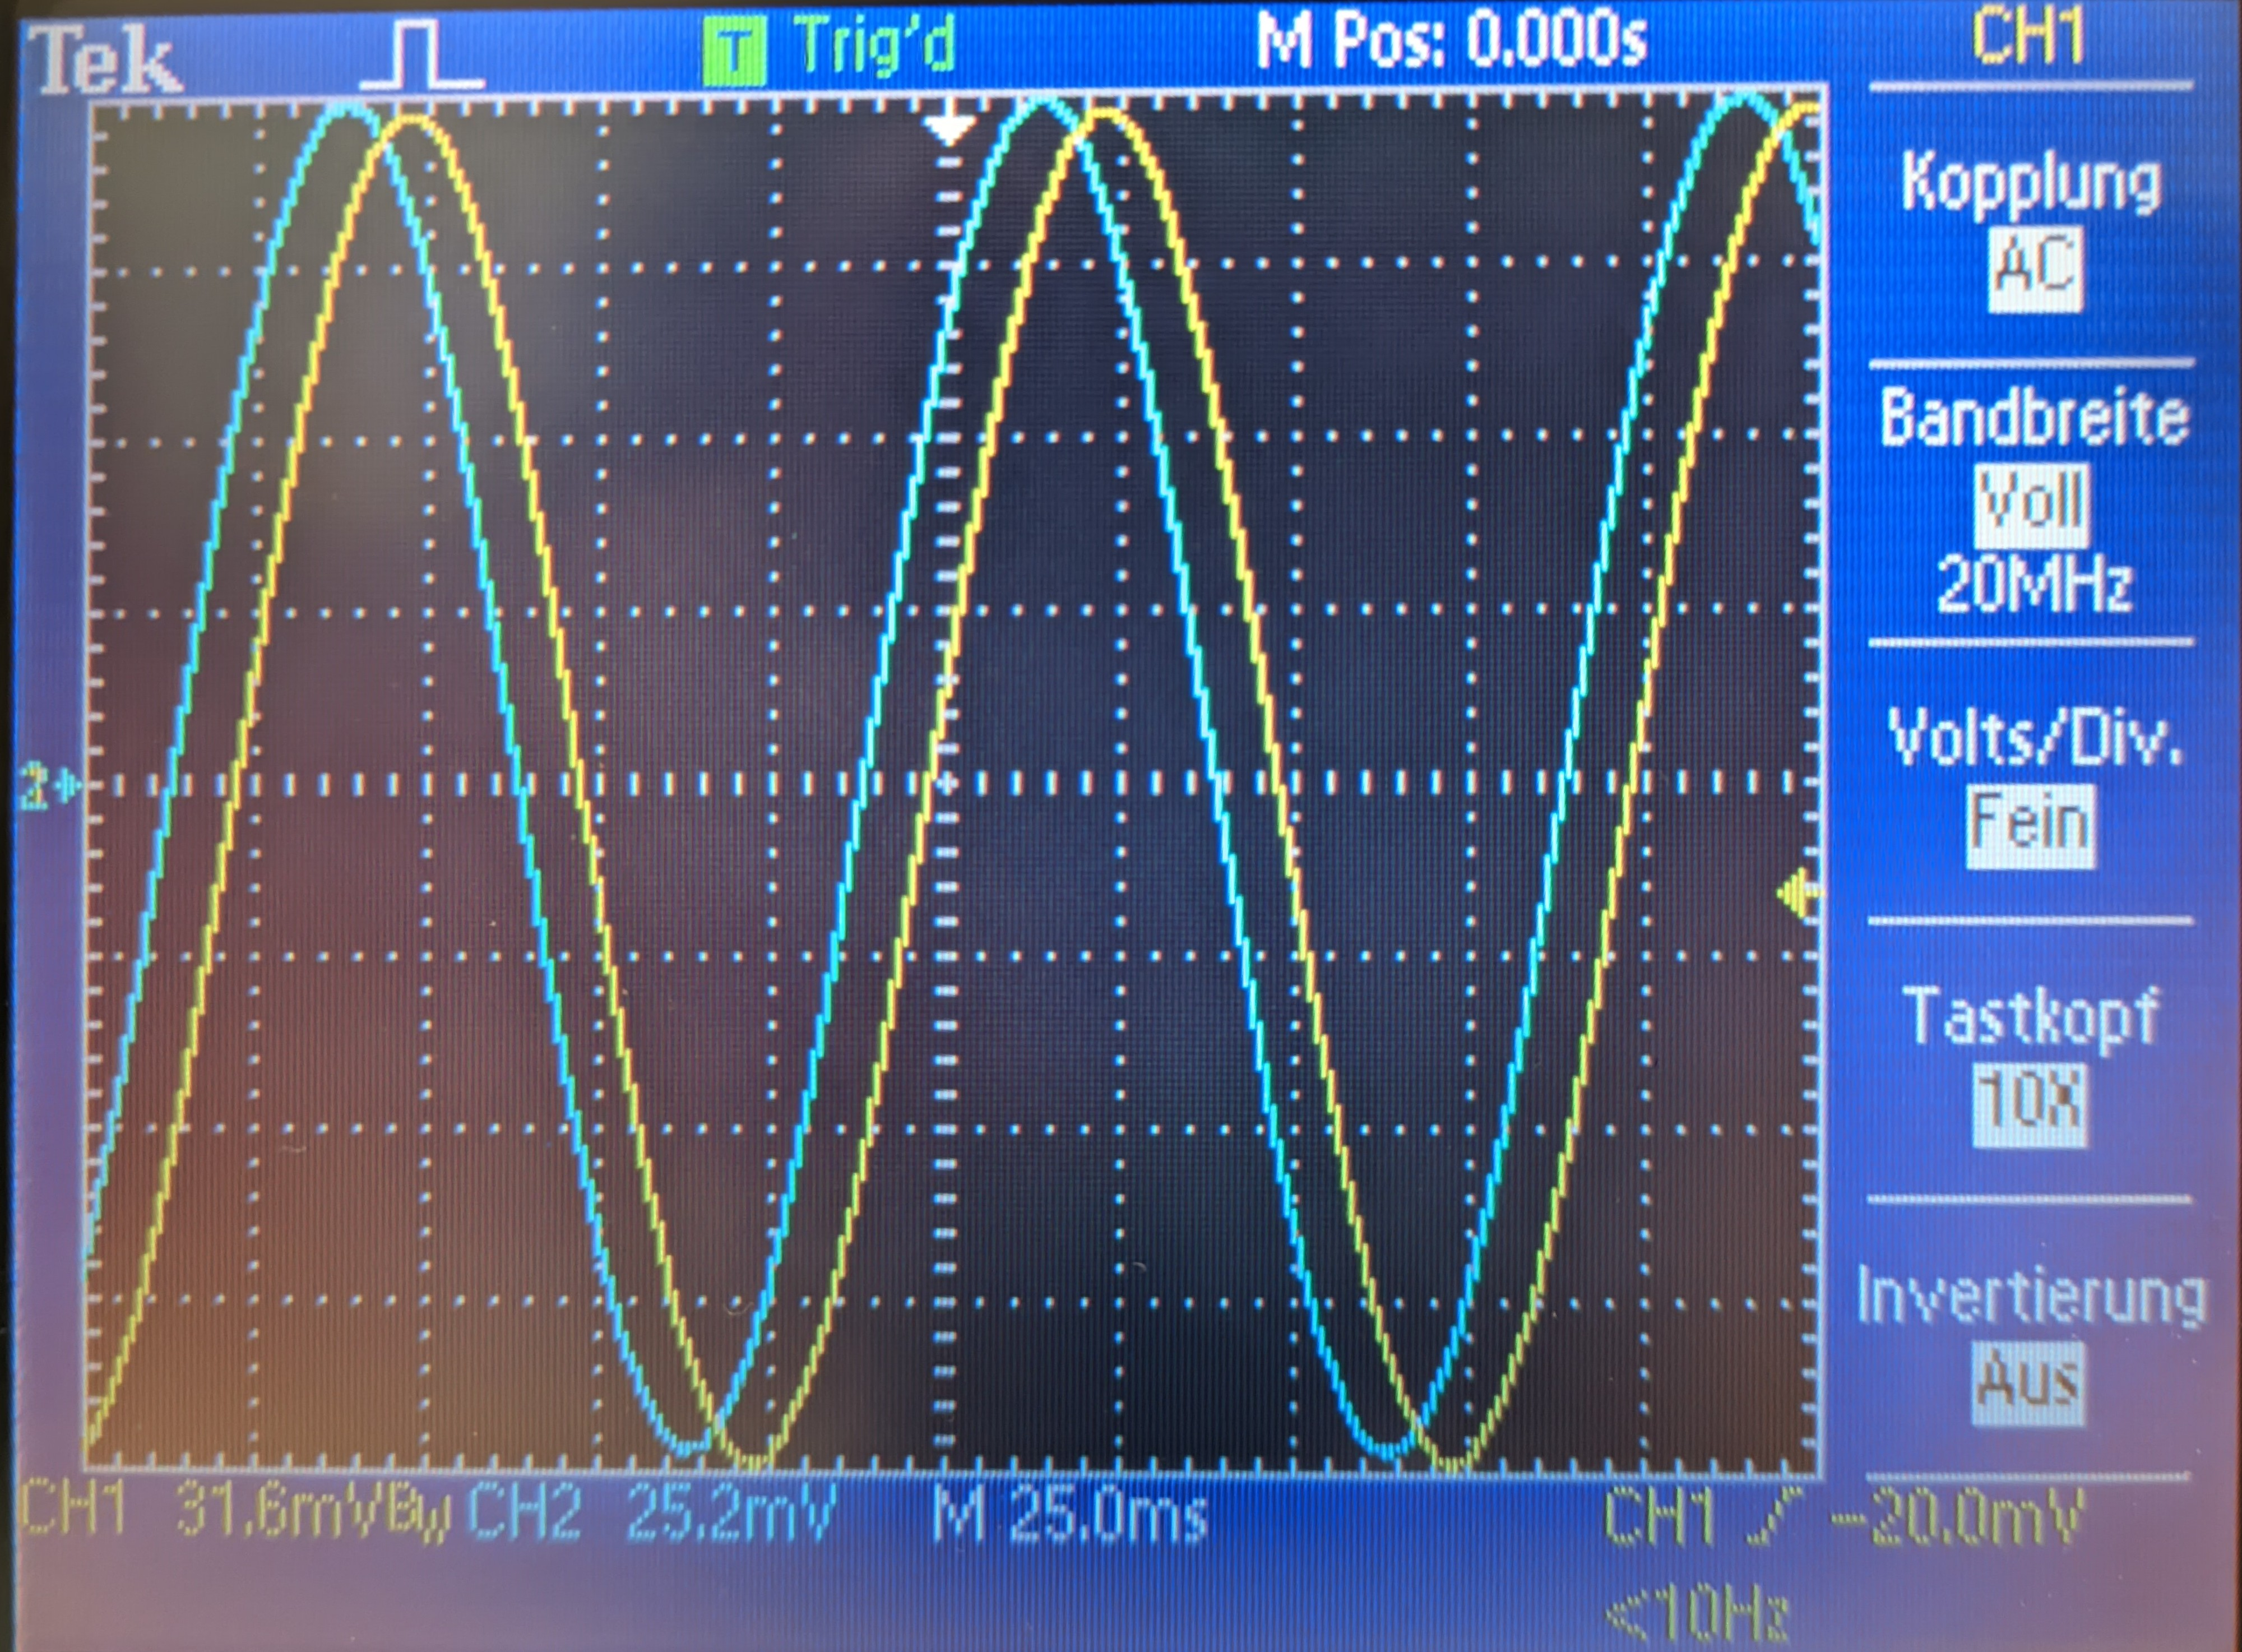
\includegraphics[width=0.95\textwidth]{./figures/integrator/sinussignal.jpg}
  \caption{}
  \label{fig:mess_integrator_sinussignal}
\end{figure}

\begin{figure}[H]
  \centering
    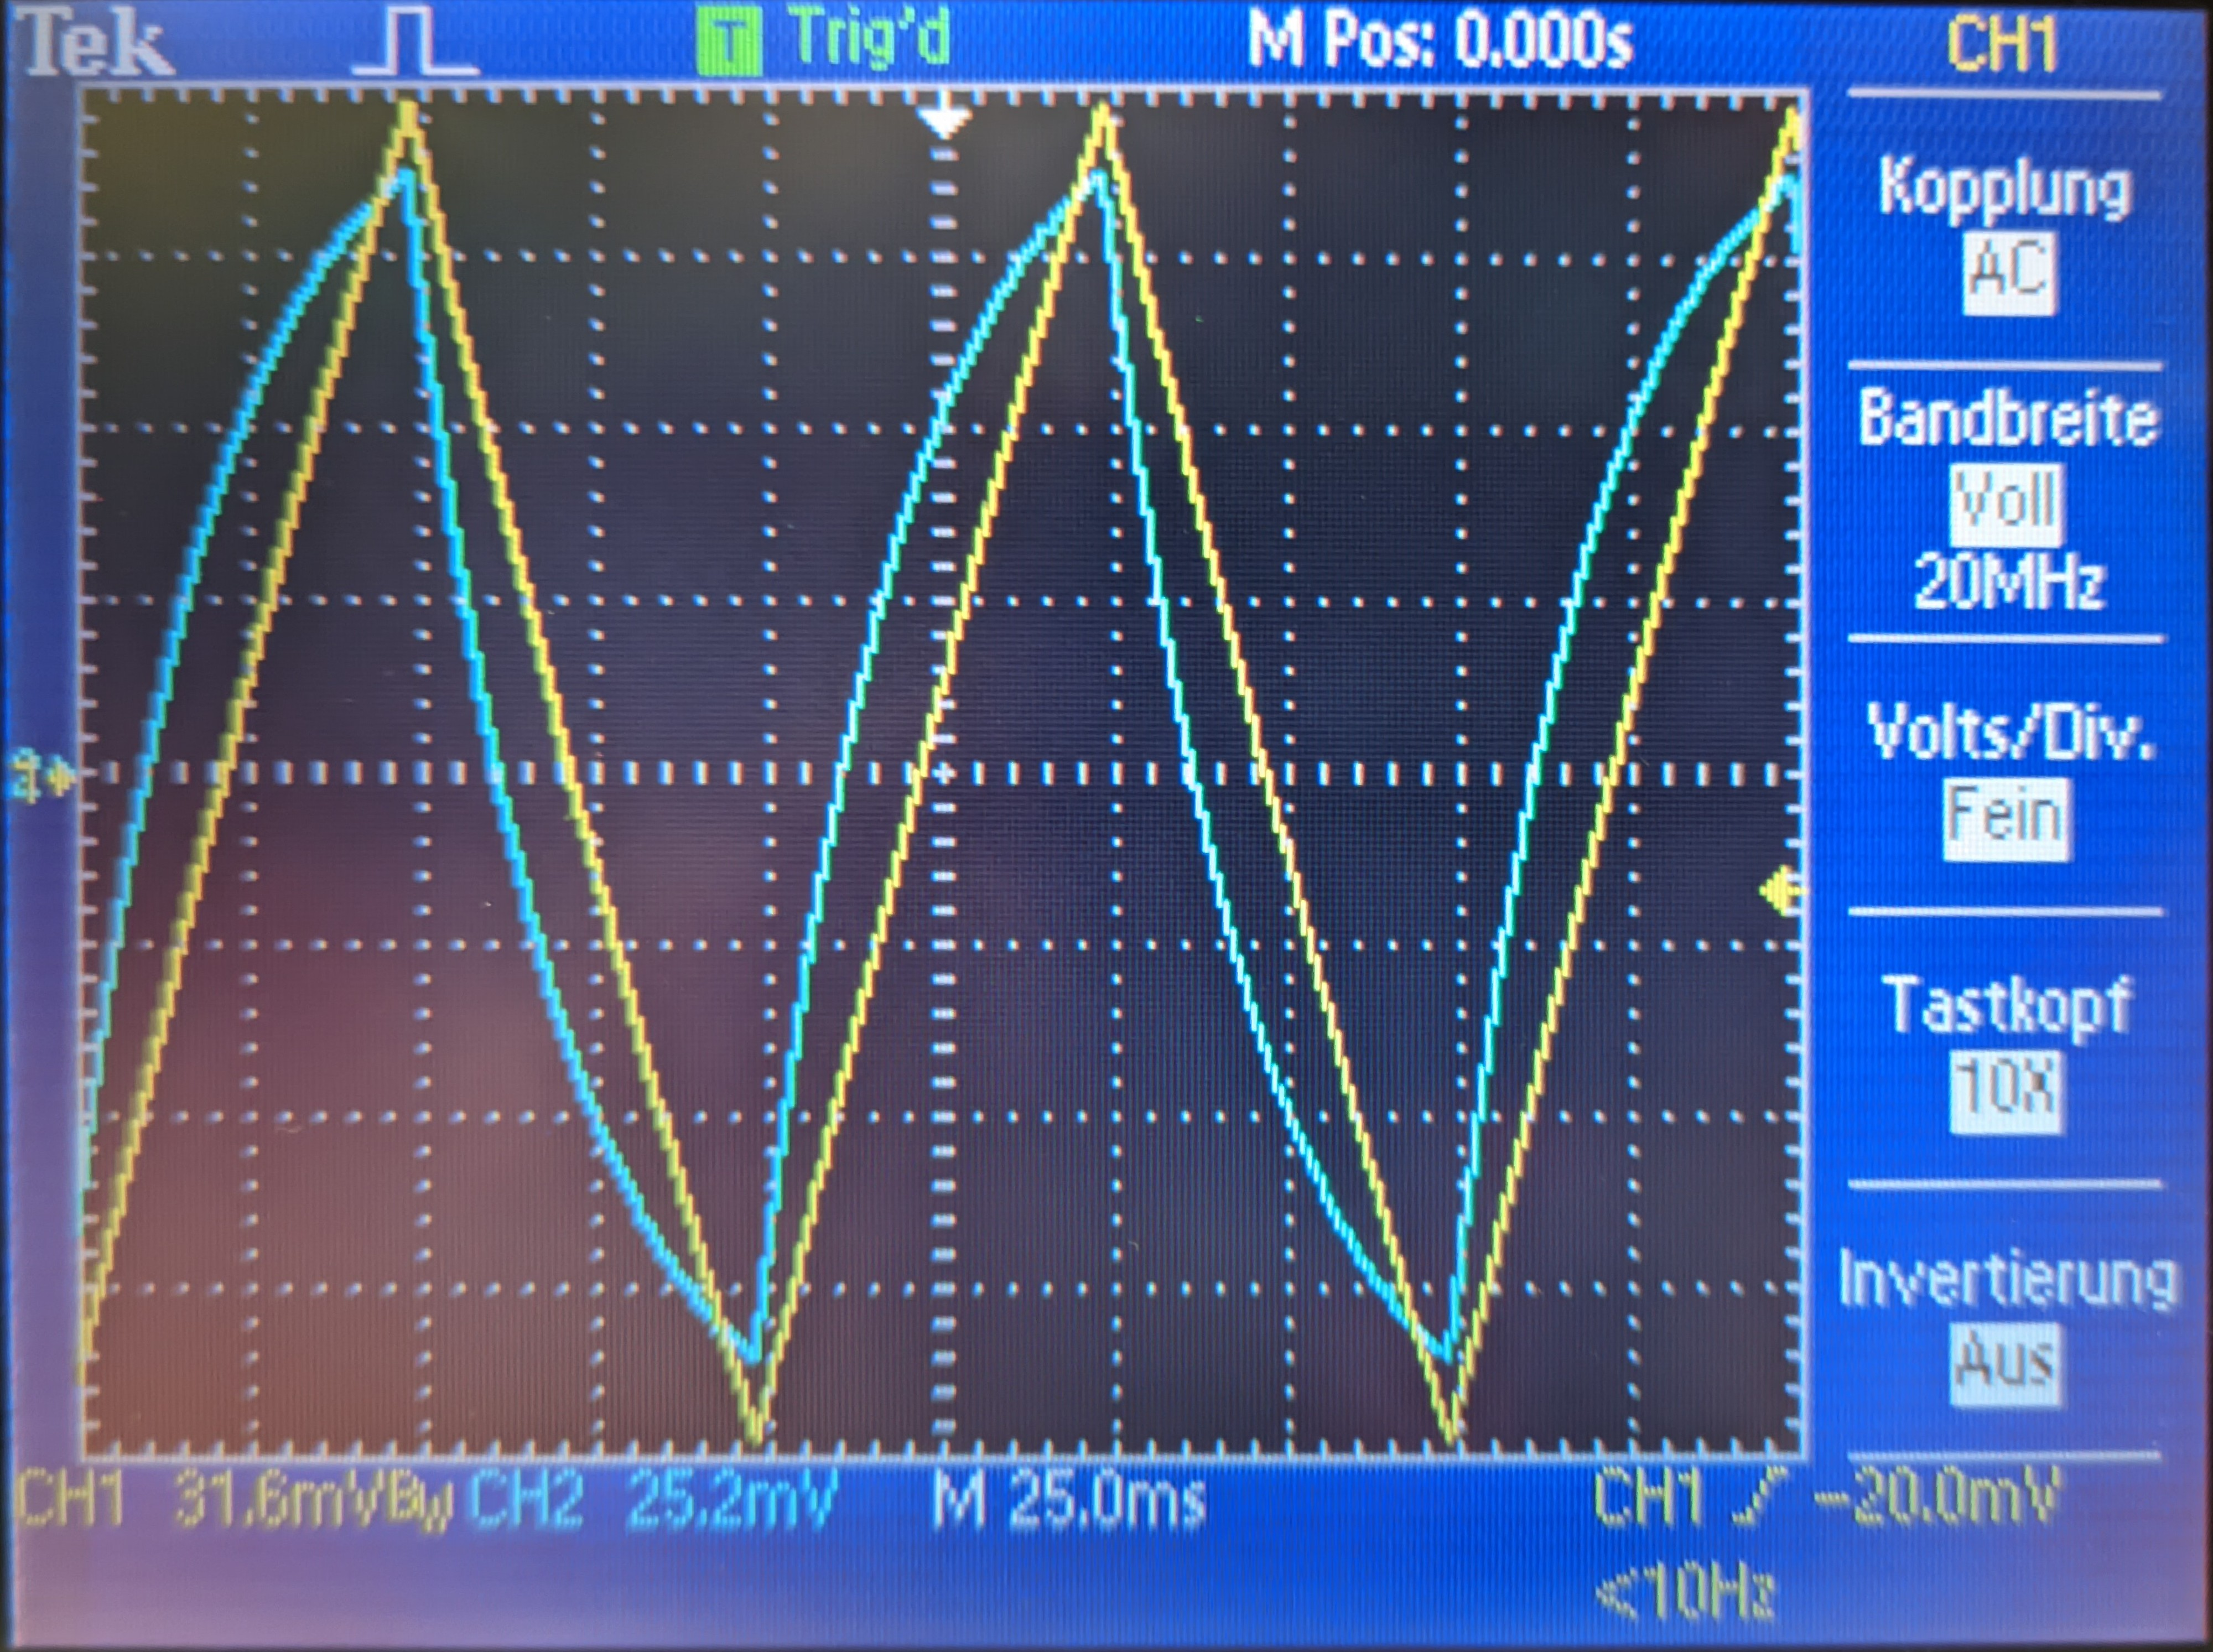
\includegraphics[width=0.95\textwidth]{./figures/integrator/dreiecksignal.jpg}
  \caption{}
  \label{fig:mess_integrator_dreiecksignal}
\end{figure}

% NOTE: Erwaehnen Rechteckspannung konnte nicht gemacht werden.

% 8) Vergleichen Sie die frequenzabhängige Verstärkung der Schaltung in einem Bereich
% zwischen 5 und 50 Hz mit der Simulation.
\paragraph{Untersuchung der frequenzabhänigen Verstärkung}

\begin{figure}[H]
  \centering
    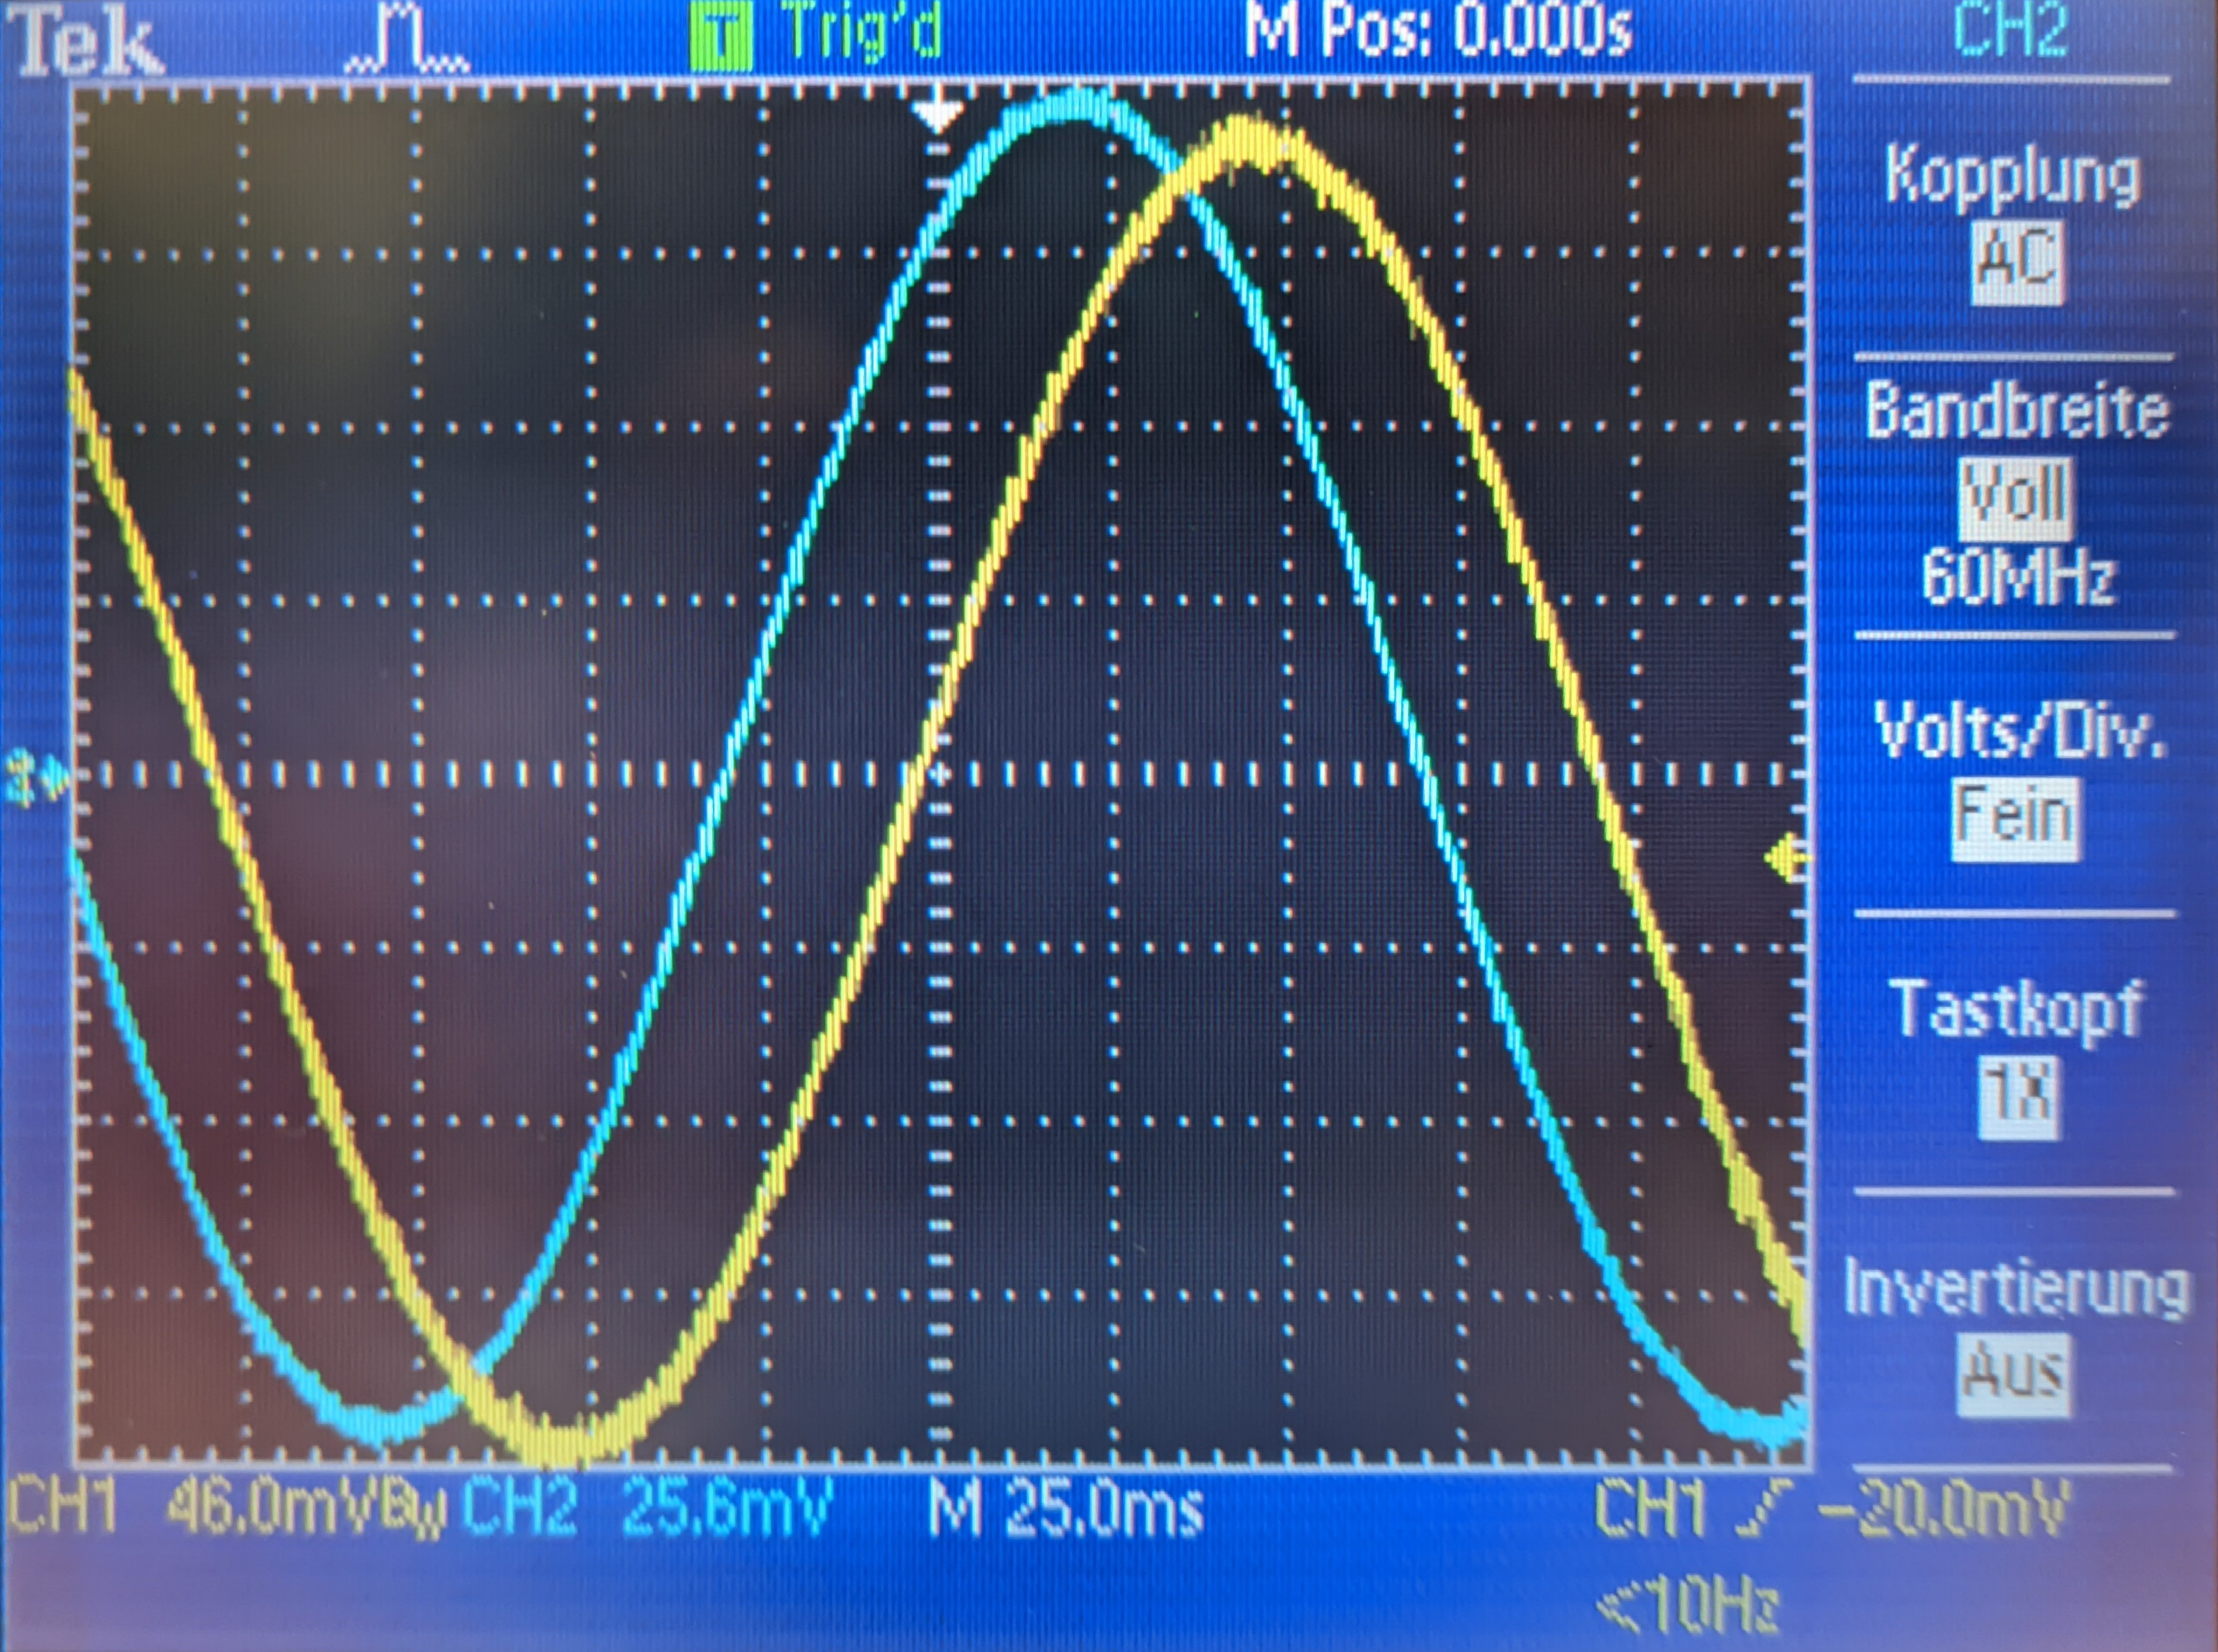
\includegraphics[width=0.95\textwidth]{./figures/integrator/5hz.jpg}
  \caption{}
  \label{fig:mess_integrator_5hz}
\end{figure}

\begin{figure}[H]
  \centering
    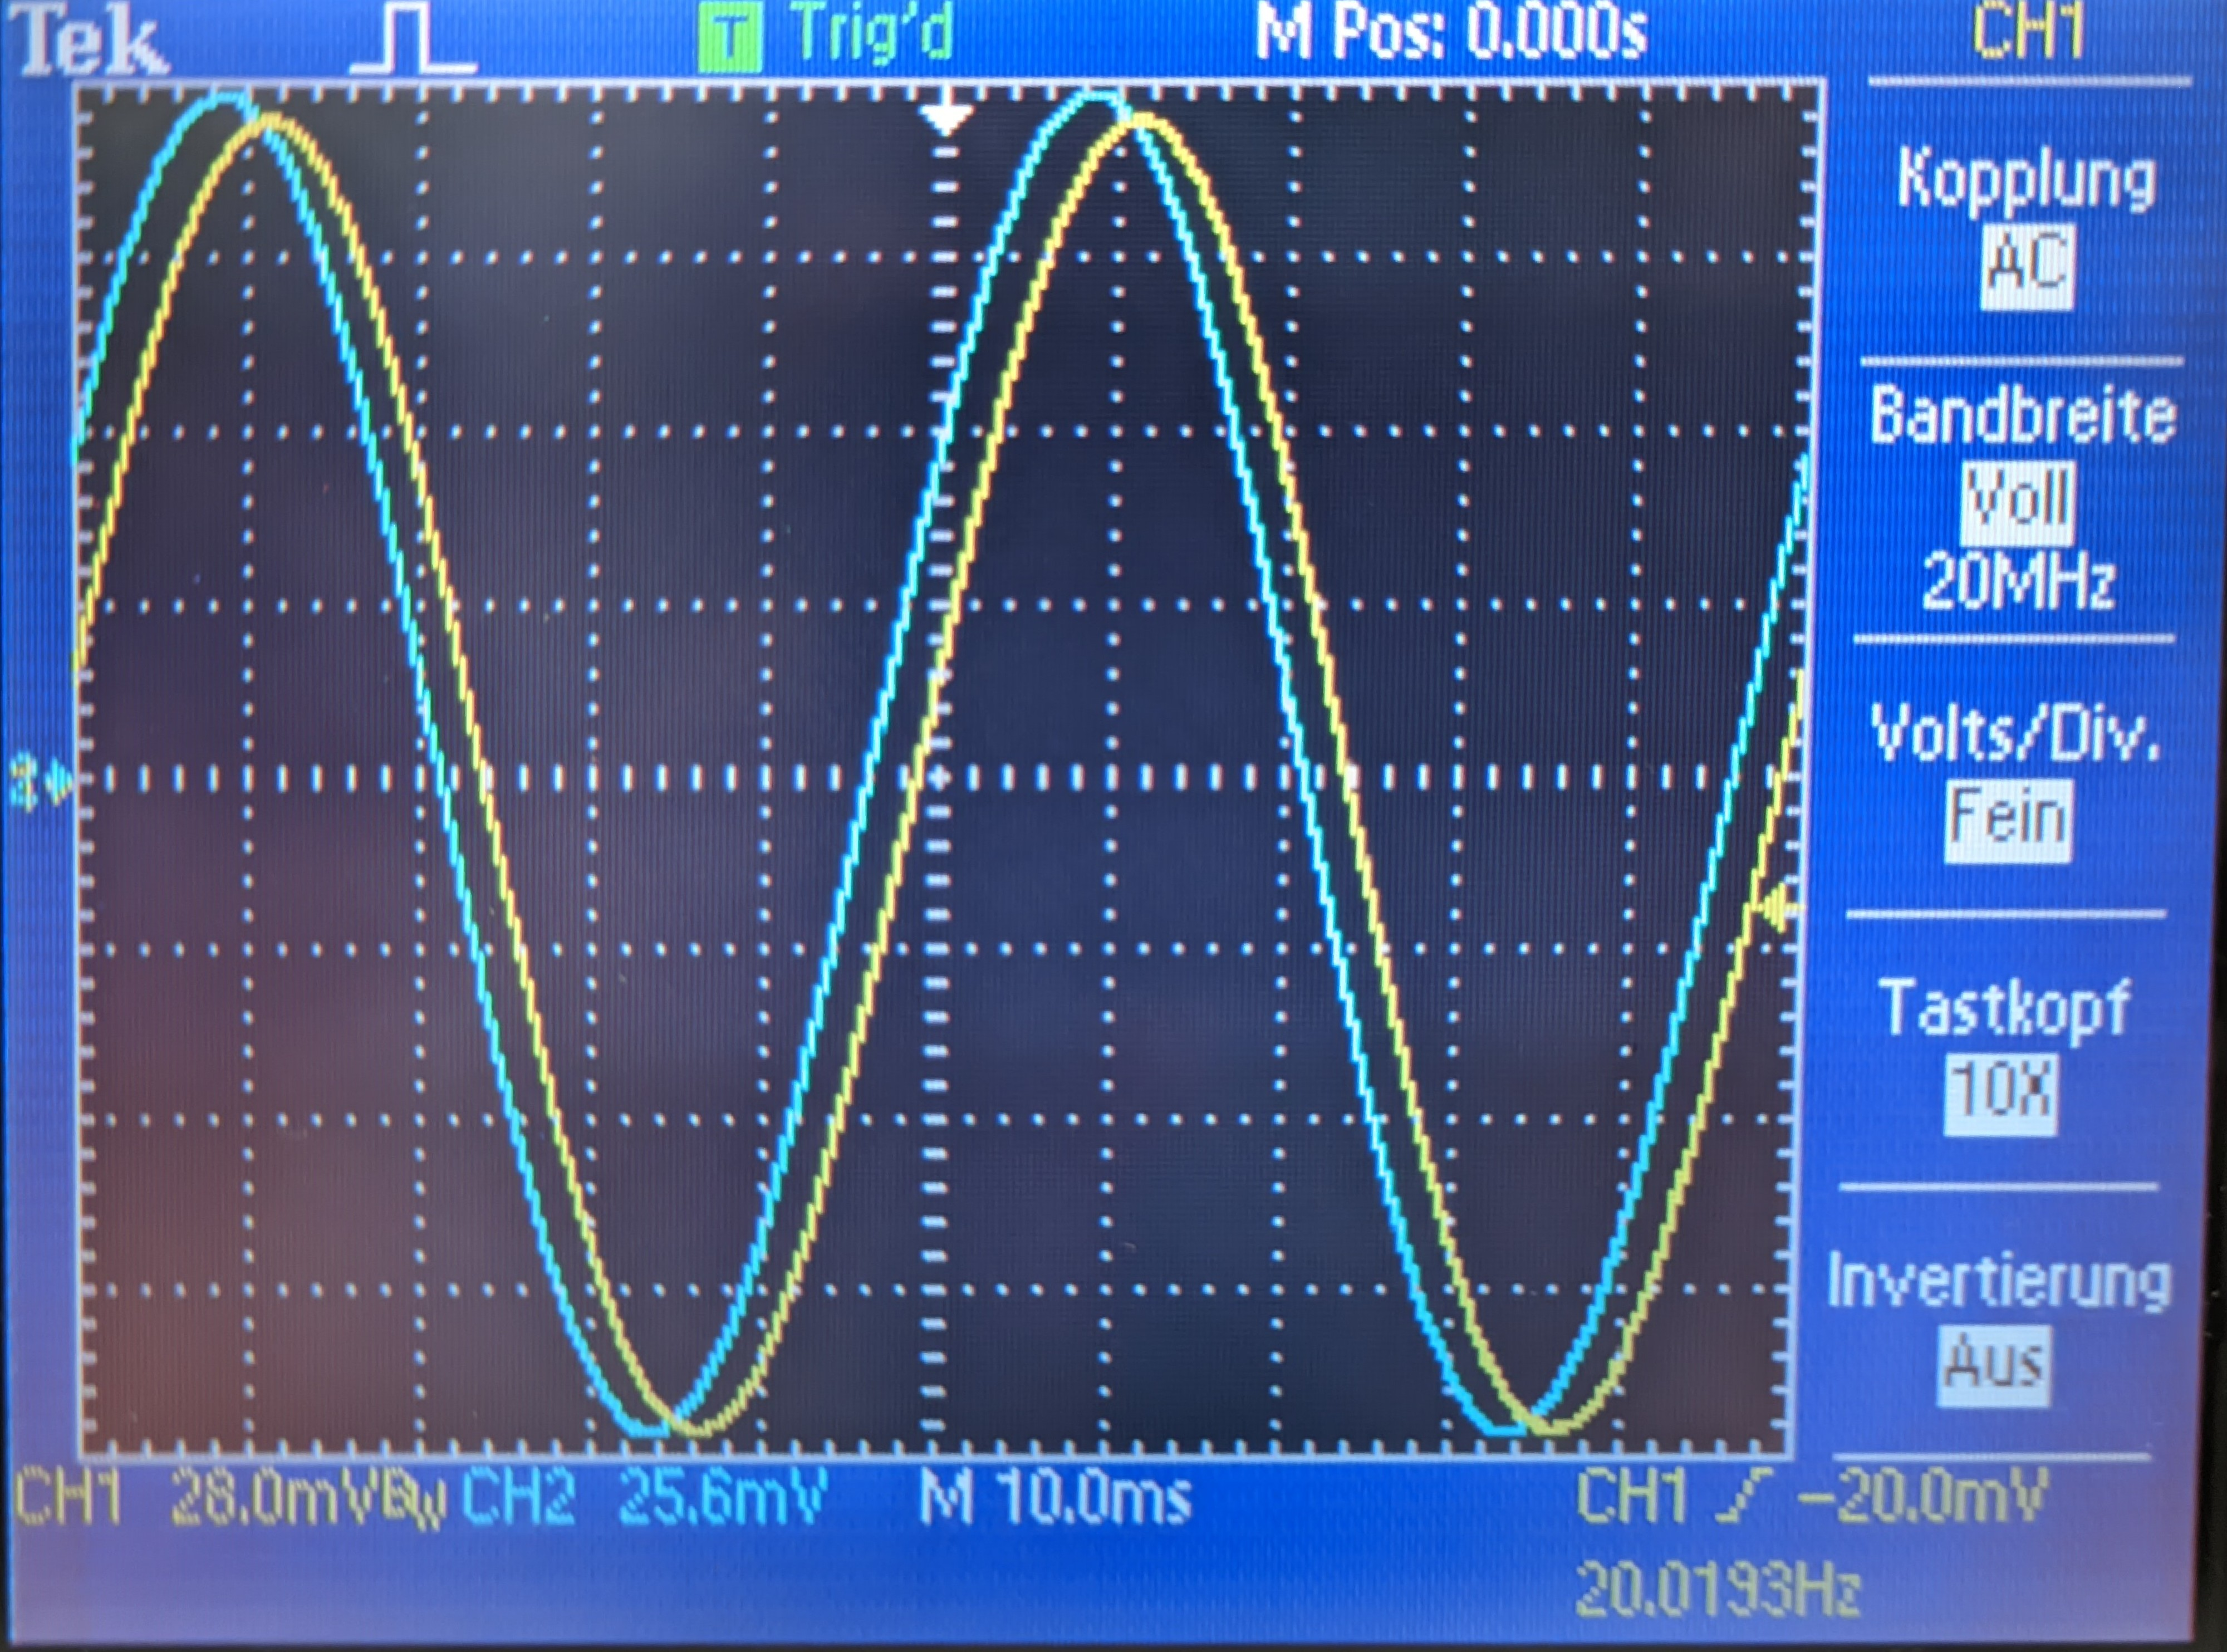
\includegraphics[width=0.95\textwidth]{./figures/integrator/20hz.jpg}
  \caption{}
  \label{fig:mess_integrator_20hz}
\end{figure}

\begin{figure}[H]
  \centering
    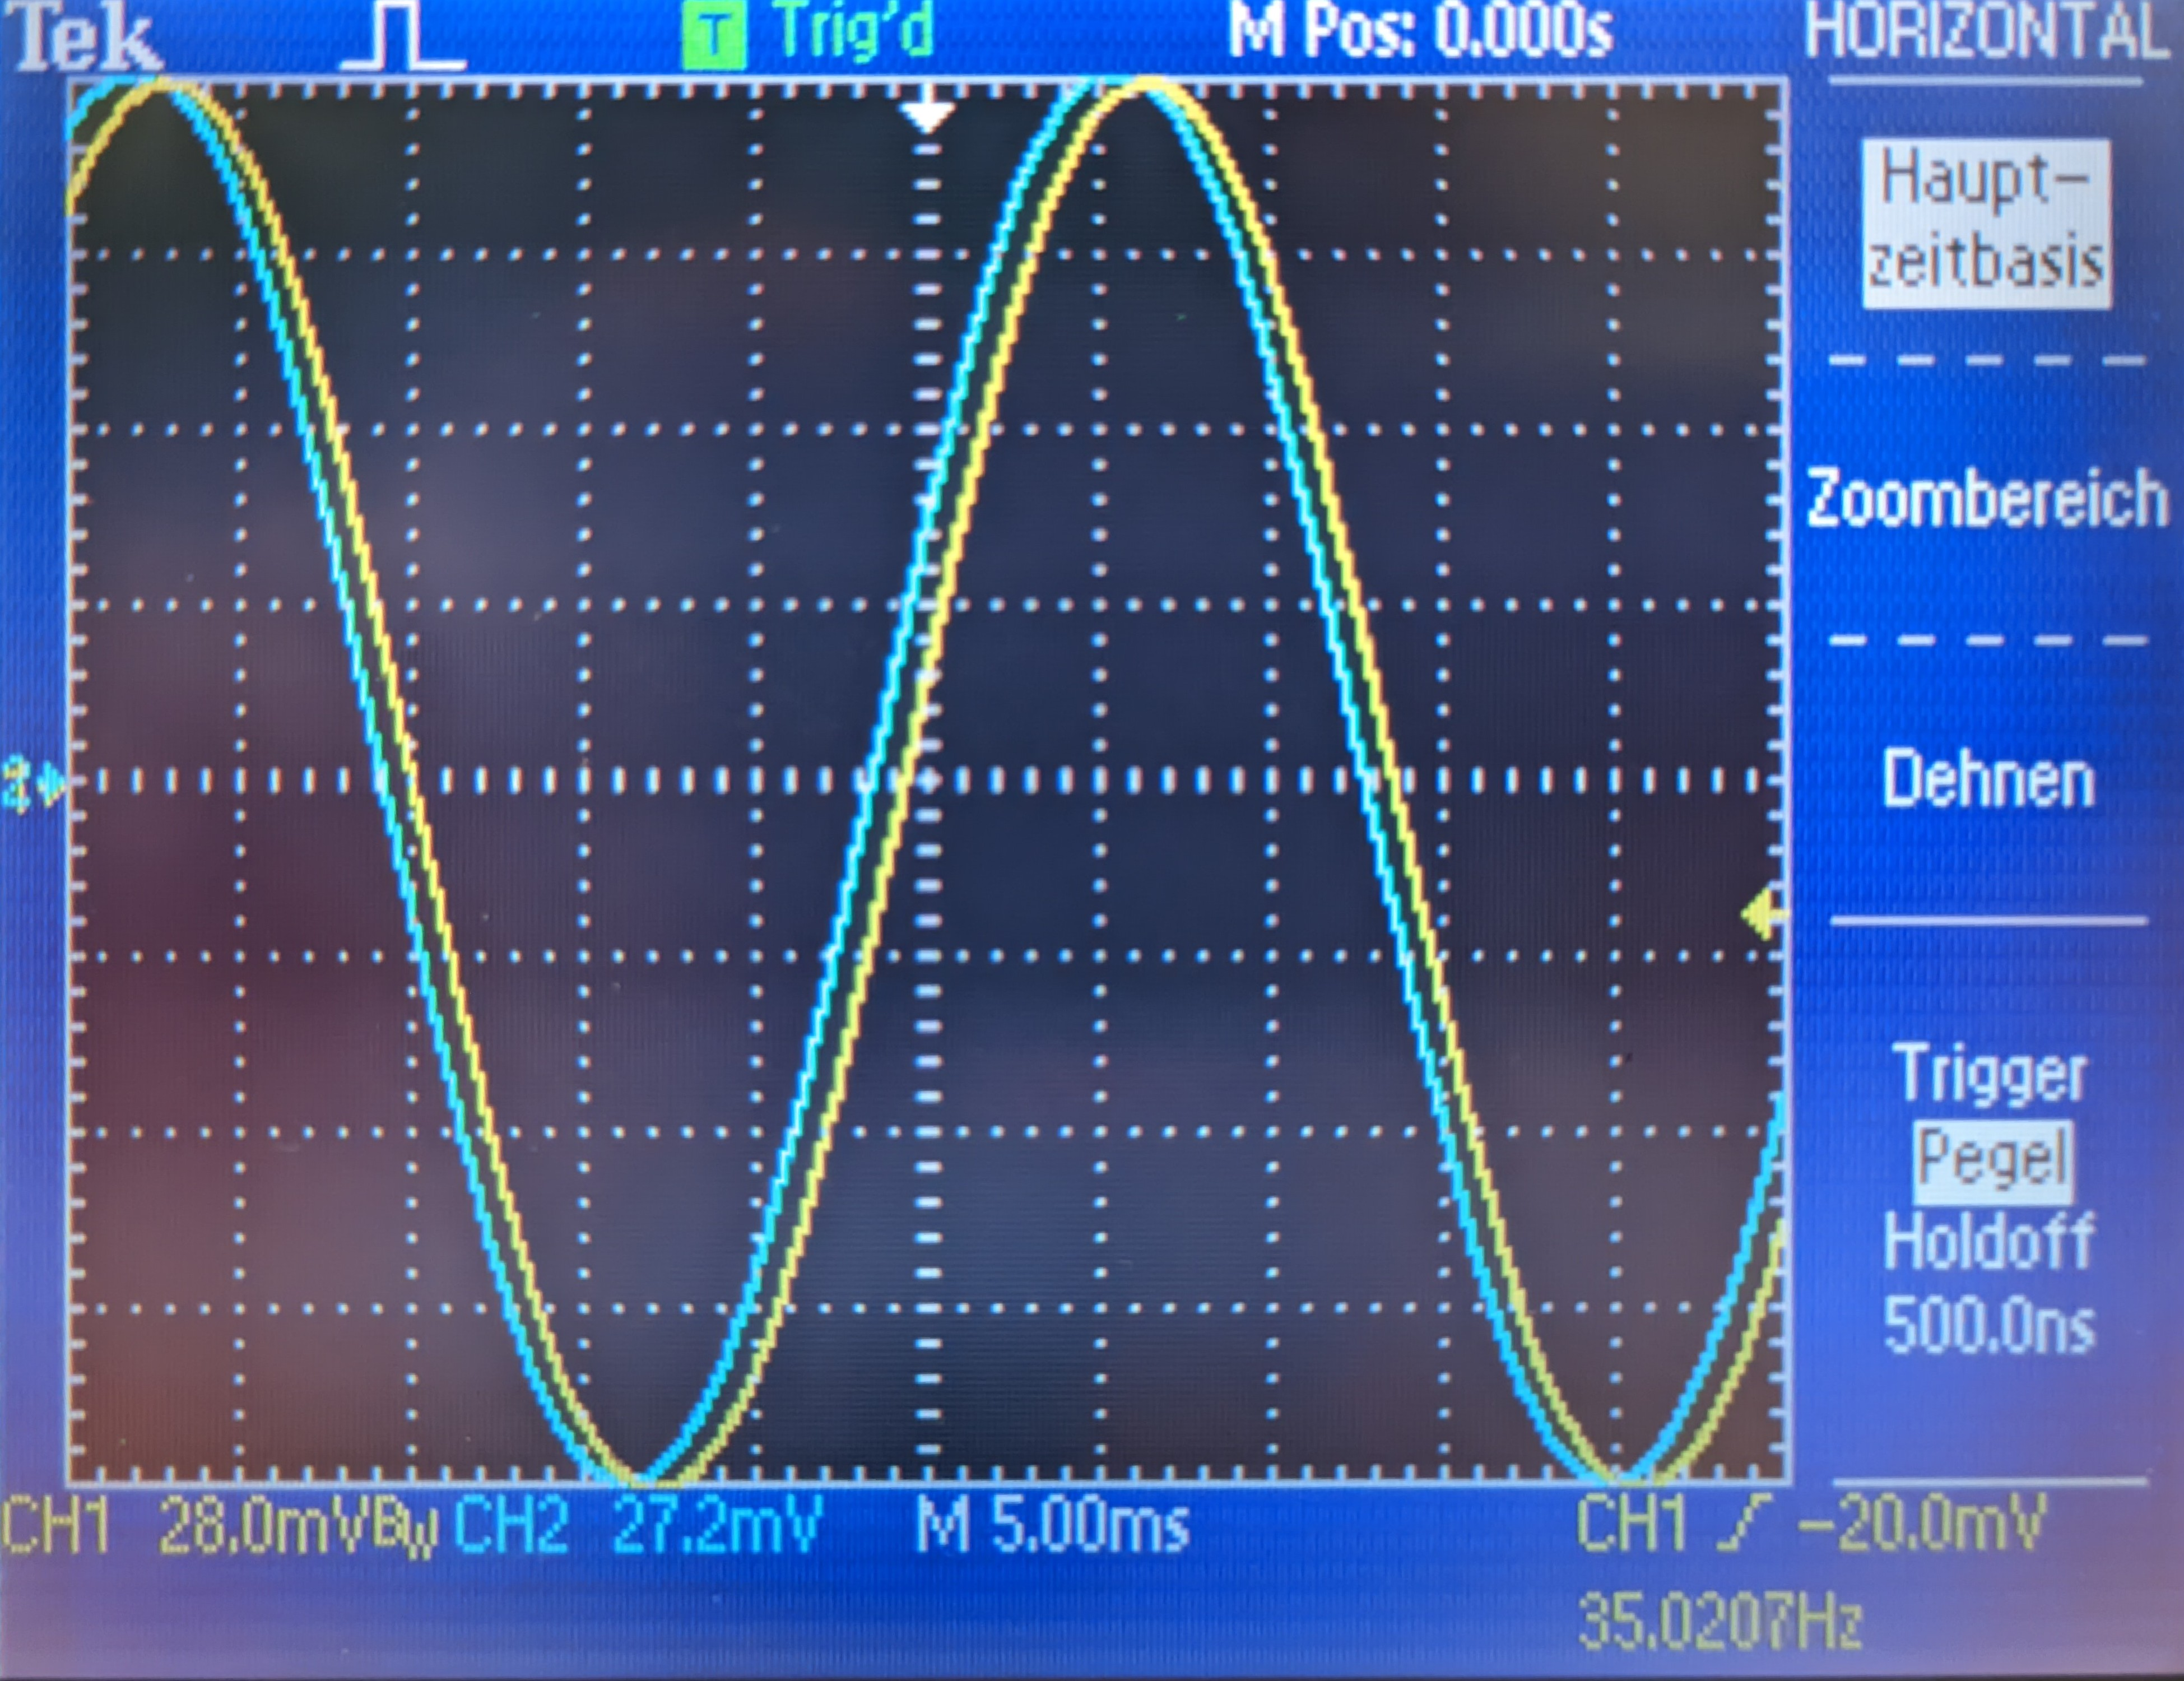
\includegraphics[width=0.95\textwidth]{./figures/integrator/35hz.jpg}
  \caption{}
  \label{fig:mess_integrator_35hz}
\end{figure}

\begin{figure}[H]
  \centering
   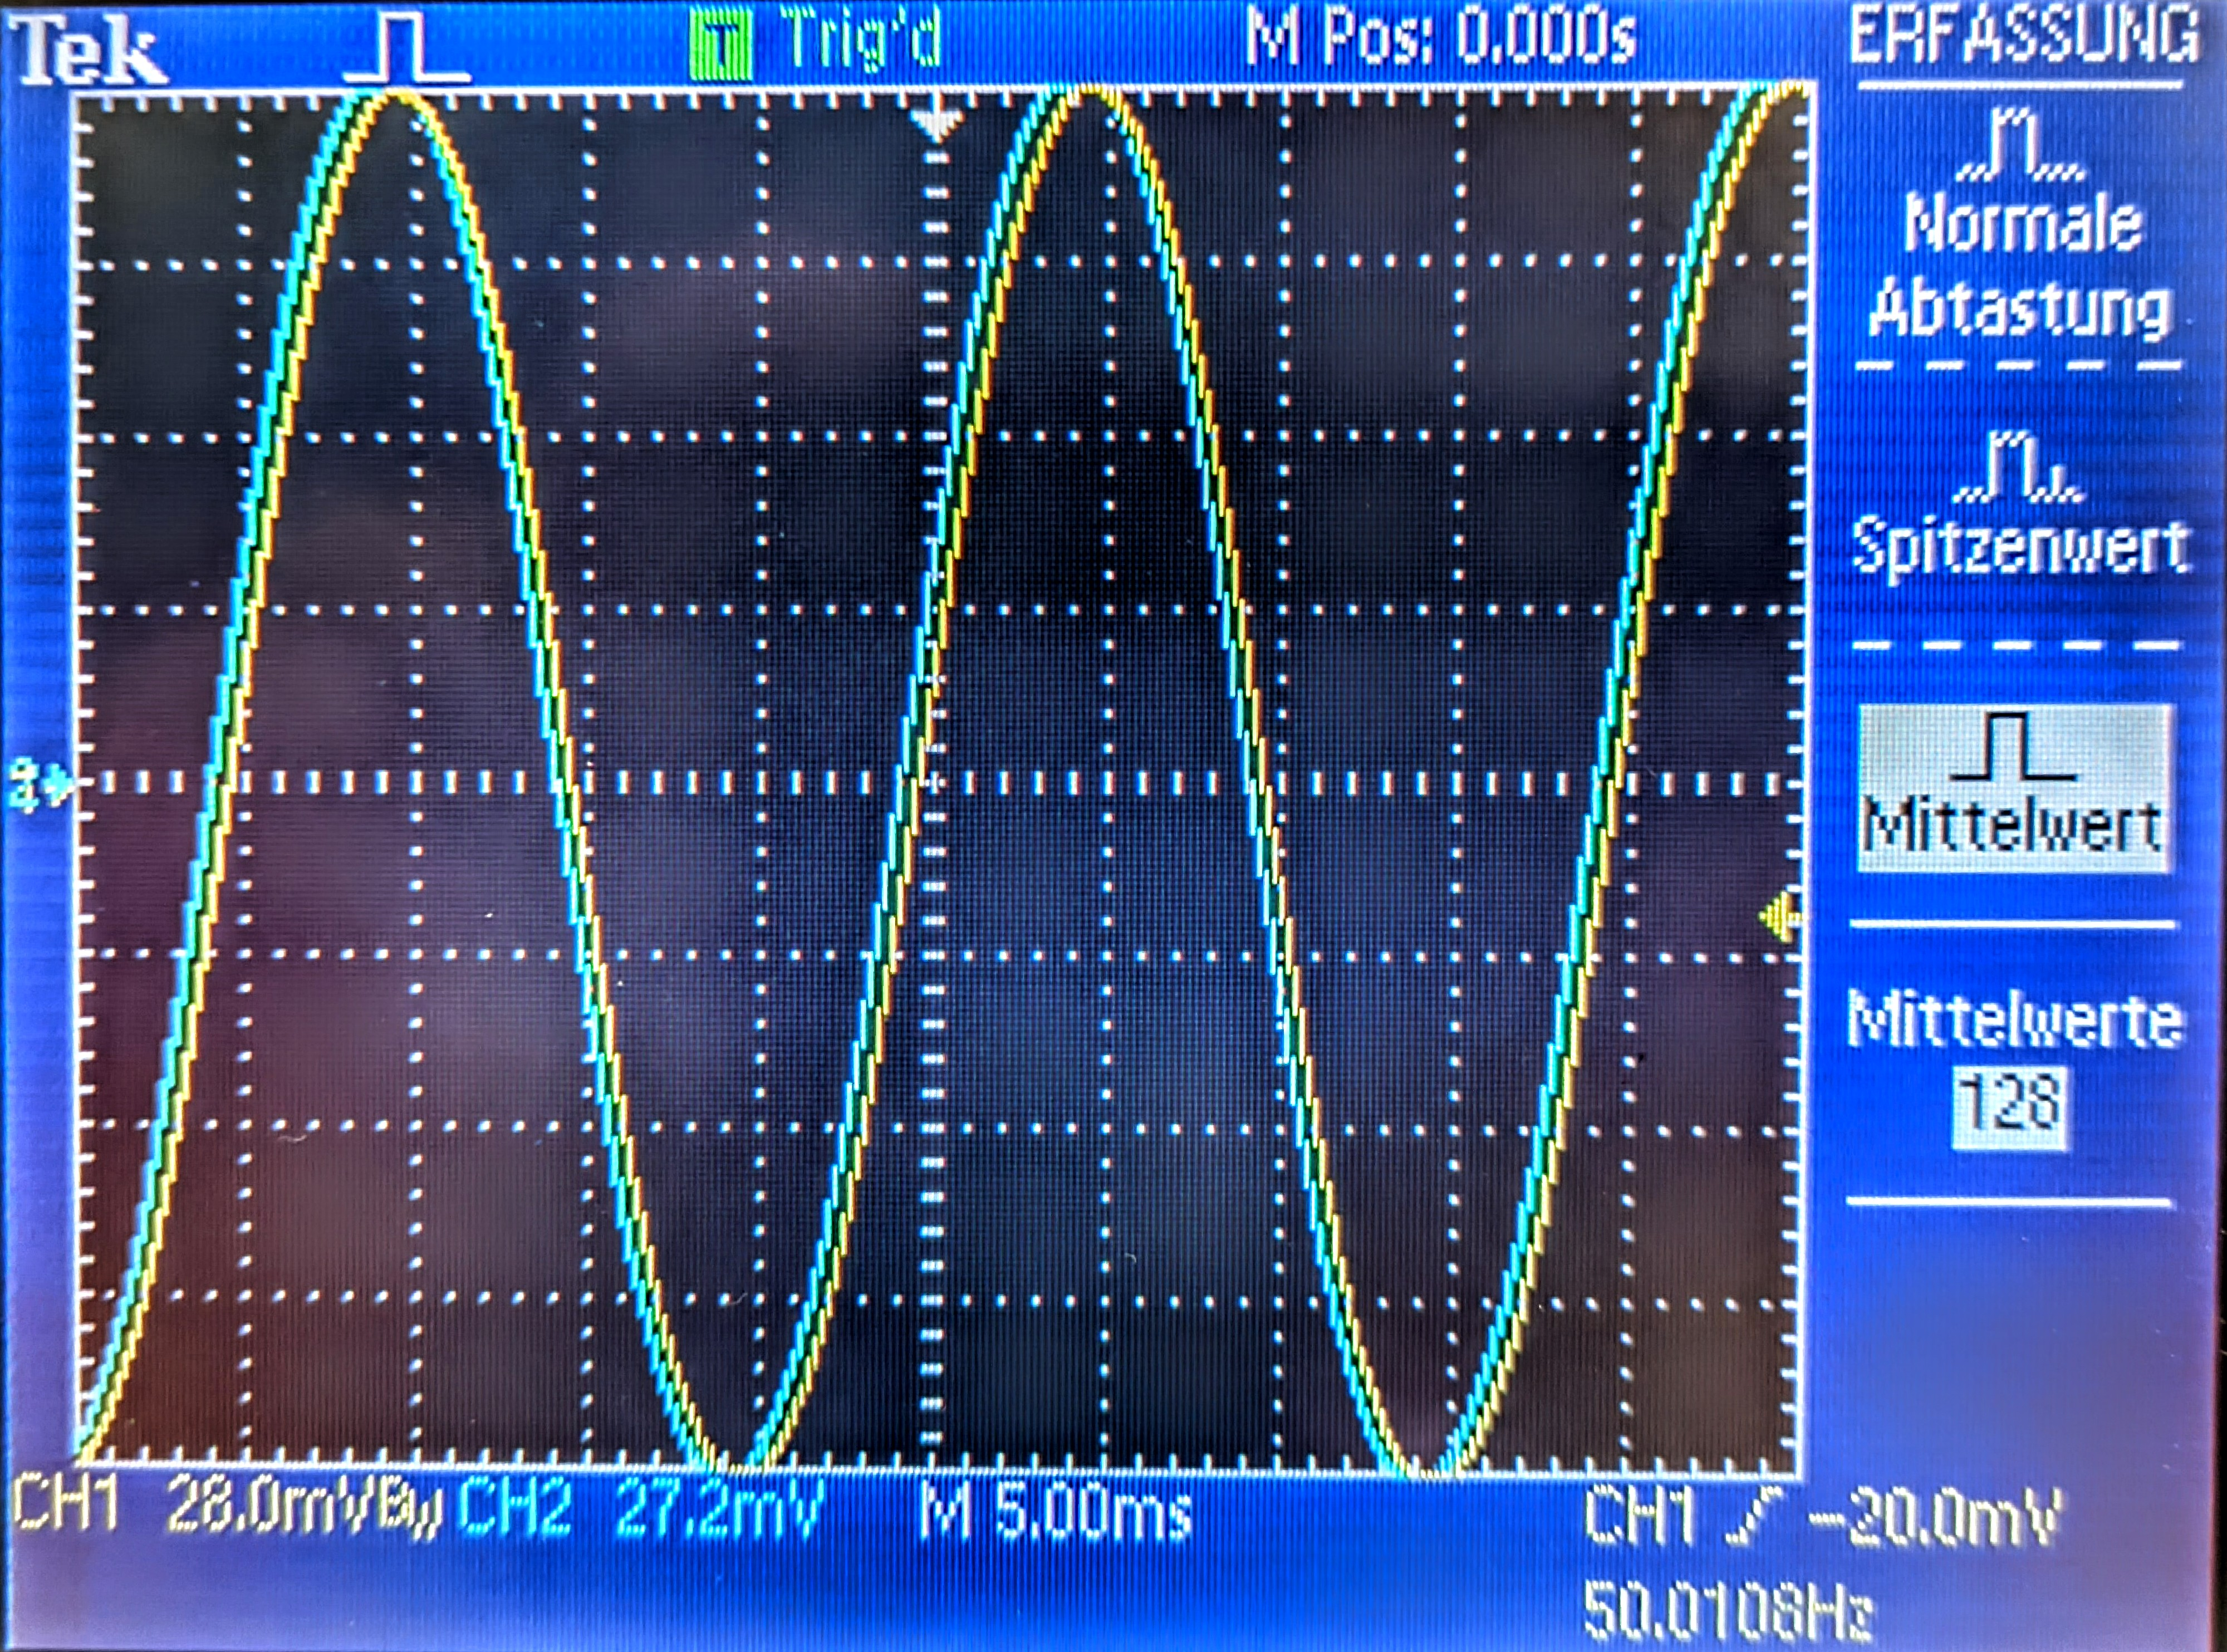
\includegraphics[width=0.95\textwidth]{./figures/integrator/50hz.jpg}
  \caption{}
  \label{fig:mess_integrator_50hz}
\end{figure}

% 9) Die Simulation ist um die genannte Verstärkerstufe zu erweitern.
% Wiederholen Sie mit der neuen Schaltung Punkt 2 und 7
\paragraph{Simulation Untersuchung der frequenzabhänigen Verstärkung}



% zu 4: Auswertung siehe EPM Skript nur Besprechung von Umformungen und 
% Sachen die man mit den Messungen machen muss damit man Conclusion und Wissen 
% gewinnen kann.
% Entsprechend der in Punkt 2. angegebenen Beziehungen (Formeln) ist aus den
% Messergebnissen in Punkt 5. das in Punkt 1. formulierte Endergebnis zu
% berechnen. Oft ist eine Ermittlung des Endergebnisses aus einer grafischen
% Darstellung bzw. eine grafische Veranschaulichung zweckmaßig. Dabei kann
% die Verwendung von Millimeterpapier oder Computerprogrammen hilfreich sein.
% Wenn eine Bearbeitung der Daten auf dem Computer erfolgt, sollte bei der
% Darstellung der Graphen eine sinnvolle Skalenteilung des Koordinatensystems
% gemacht werden. Die Unsicherheitsbetrachtung f ̈ur die angegebenen Messwerte,
% sowie fur Zwischen- und Endergebnisse ist in diesem Abschnitt
% nachvollziehbar zu beschreiben. Dabei ist nach Kapitel 1 vorzugehen und
% insbesondere auf die Klassifizierung der Unsicherheit (Typ-A/B) und die
% Unsicherheitsfortpflanzung einzugehen.
\section{Auswertung}\label{sec:Auswertung}

\subsection{Simulation}

\subsection{Steckbrett}

% zu 5: Diskussion und Zusammenfassung
% In der Zusammenfassung stehen noch einmal die wichtigsten Messergebnisse, wobei auf Tabellen und
% Abbildungen nur verwiesen werden soll. Die Ergebnisse sind auch zu diskutieren. Insbesondere müssen
% Abweichungen zwischen Simulation und praktischer Durchführung diskutiert werden.
\section{Diskussion und Zusammenfassung}\label{sec:Diskussion} 
\subsection{Diskussion}
% TODO discuss the discreptency in the time measurement with the expected result 

%Es wäre wohl vernünftiger gewesen, die Schaltung an der Steckplatine zunächst aufzubauen, um etwaige 
%Ungenauigkeiten durch die Widerstände 
\subsection{Zusammenfassung}

\newpage

\printbibliography

\listoffigures

\listoftables



\end{document}
